%% Placeholder for chapter on convexity

%Below are notes for Oct23
\section{Linear/affine/convex/conic hulls \& sets}
Given a set of points $x^{(i)} \in \reals^n$, $i\in [m]$
\begin{equation*}
P = \{x^{(1)}, x^{(2)}\ldots, x^{(m)} \}
\end{equation*}

Consider combinations of form $\sum^m_{i=1} \lambda_i x^{(i)}$,

1) The "linear" hull: 

\begin{equation*}
\{x|x = \sum^m_{i=1} \lambda_i x^{(i)}, \lambda_i\in \reals, \forall i\in [m] \}
\end{equation*}

2) The "affine" hull: 

\begin{equation*}
\{x|x = \sum^m_{i=1} \lambda_i x^{(i)}, \lambda_i\in \reals, \sum^n_{i=1}\lambda_i = 1 \}
\end{equation*}


3) The "convex" hull: 

\begin{equation*}
\{x|x = \sum^m_{i=1} \lambda_i x^{(i)}, \lambda_i\in \reals, \lambda_i \geq 0, \sum^m_{i=1}\lambda_i = 1 \}
\end{equation*}


4) The "conic" hull: 

\begin{equation*}
\{x|x = \sum^m_{i=1} \lambda_i x^{(i)}, \lambda_i\in \reals, \lambda_i \geq 0 \}
\end{equation*}

Summary
\begin{center}
	\begin{tabular}{|c|c|c|}
	\hline  
   & $\lambda_i \geq 0$   & $\sum^m_{i=1}\lambda_i = 1$ \\
	\hline  
Linear&  no  & no \\
	\hline  
Affine&  no  &yes  \\
	\hline 
Covex&  yes  & yes \\
	\hline  
Conic&  yes  &  no\\
	\hline 
\end{tabular}
\end{center}


\begin{example}[Linear Hull]
	
Let $P = \{x^{(1)}, x^{(2)} \}$, linear hull of $P = \text{span}\{x^{(1)},\ldots,x^{(m)} \} =\text{span}(P)$.

Note that linear hull of $P$ forms the smallest subspace that contains $P$.

\end{example}

\begin{example}[Affine Hull]
Let $P = \{x^{(1)}, x^{(2)} \}$, the point of the affine hull is given by
\begin{align*}
x 
&= \lambda_1x^{(1)} + \lambda_2x^{(2)}\\
&= \lambda_1x^{(1)} + (1-\lambda)_1x^{(1)}\\
&= x^{(2)} + \lambda(x^{(1)} - x^{(2)})
\end{align*}
Hence, $\text{aff}(P) = x^{(2)} + \text{span}(x^{(1)} - x^{(2)})$.

\vspace{0.3cm}
Let $P = \{x^{(1)}, x^{(2)}, x^{(3)} \}$, the point of the affine hull is given by
\begin{align*}
x 
&= \lambda_1x^{(1)} + \lambda_2x^{(2)} + \lambda_3x^{(3)}\\
&= (1 - \lambda_2 - \lambda_3)x^{(1)} + \lambda_2x^{(2)} + \lambda_3x^{(3)}\\
&= x^{(1)} + \lambda_2(x^{(2)} - x^{(1)}) + \lambda_3(x^{(3)} - x^{(1)})
\end{align*}
Hence,  $\text{aff}(P) = x^{(1)} + \text{span}(x^{(2)} - x^{(1)}) + \text{span}(x^{(3)} - x^{(1)})$.

Note that, the affine hull is the smallest affine set contains the set $P$.

\begin{marginfigure}
	\centering
	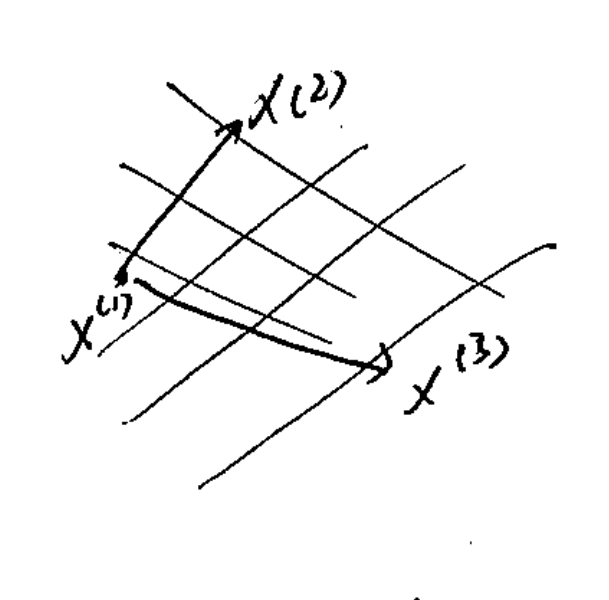
\includegraphics[width=1.8in,height=1.8in]{figures/ch08/figure1023_1.png}
	%\caption{This is an inserted JPG graphic} 
	%\label{fig:graph} 
\end{marginfigure}

\end{example}


\begin{example}[Convex hull]
Let $P = \{x^{(1)},  x^{(2)}\}$, the point of convex hull is given by 
\begin{align*}
x 
&= \lambda_1x^{(1)} + \lambda_2x^{(2)}\\
&= (1-\lambda)x^{(1)} + \lambda x^{(2)}\\
&= x^{(1)} + \lambda(x^{(2)} - x^{(1)})
\end{align*}

\vspace{0.3cm}
Let $P = \{x^{(1)},  x^{(2)}, x^{(3)} \}$, the point of convex hull is given by 
\begin{align*}
x 
&= \lambda_1x^{(1)} + \lambda_2x^{(2)} + \lambda_3x^{(3)}\\
&= x^{(1)} + \lambda_2(x^{(2)} - x^{(1)}) + \lambda_3(x^{(3)} - x^{(1)})\\
&= x^{(1)} + \lambda \gamma(x^{(2)} - x^{(1)}) + (1 - \lambda)\gamma(x^{(3)} - x^{(1)})
\end{align*}


\begin{marginfigure}
	\centering
	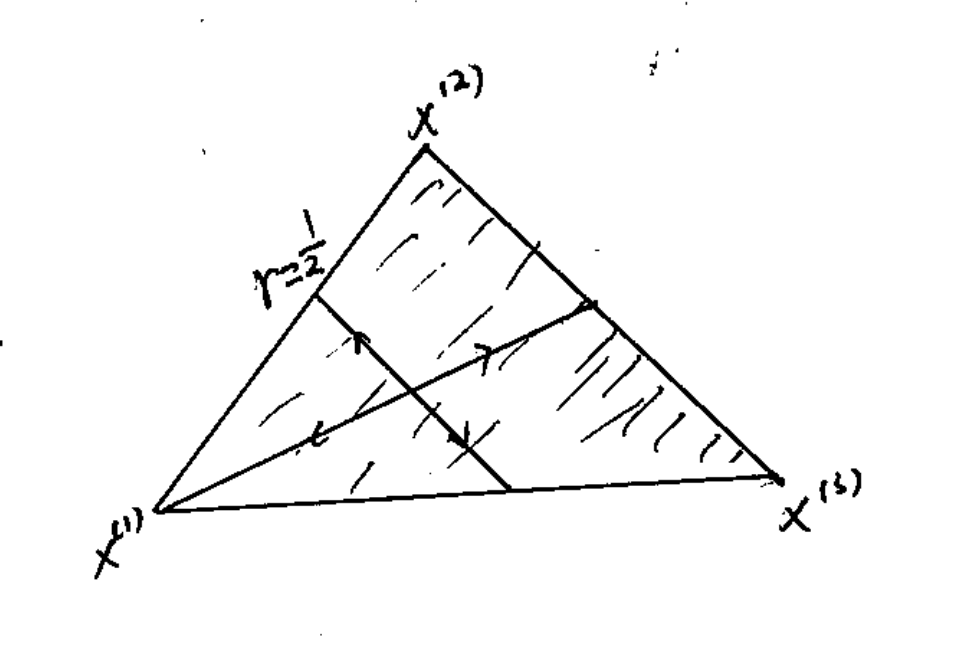
\includegraphics[width=1.8in,height=1.8in]{figures/ch08/figure1023_2.png}
	%\caption{This is an inserted JPG graphic} 
	%\label{fig:graph} 
\end{marginfigure}

\begin{marginfigure}
	\centering
	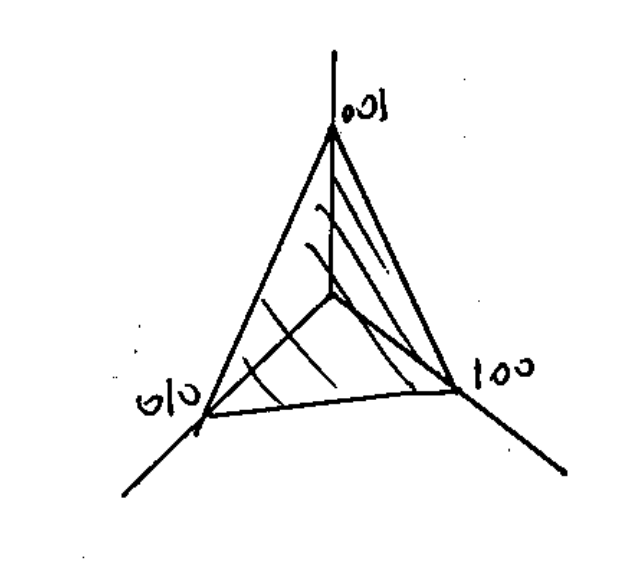
\includegraphics[width=1.8in,height=1.8in]{figures/ch08/figure1023_3.png}
	%\caption{This is an inserted JPG graphic} 
	%\label{fig:graph} 
\end{marginfigure}

\end{example}


\begin{example}[Conic hull]
Let $P = \{x^{(1)}, x^{(2)} \}$, the point of conic hull is given by 
\begin{align*}
x 
&= \lambda_1x^{(1)} + \lambda_2x^{(2)}\\
&= ( \lambda_1 + \lambda_2)[\frac{\lambda_1}{\lambda_1 + \lambda_2}x^{(1)} + \frac{\lambda_2}{\lambda_1 + \lambda_2}x^{(2)}]\\
&= \gamma[\lambda x^{(1)} + (1-\lambda)x^{(2)}]
\end{align*}

\begin{marginfigure}
	\centering
	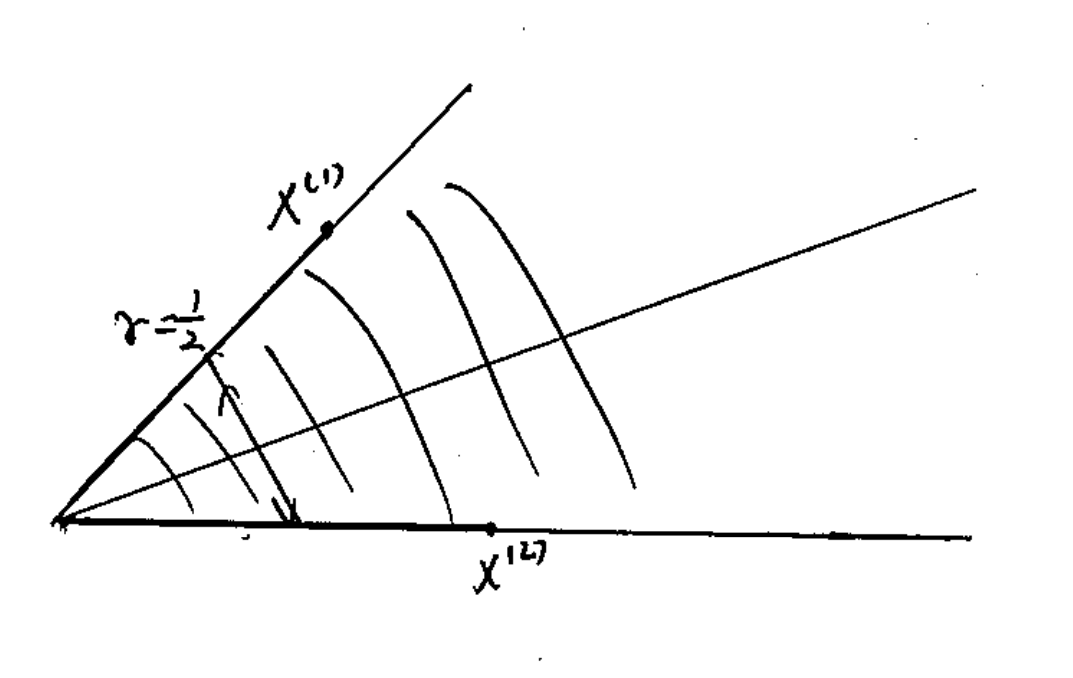
\includegraphics[width=1.8in,height=1.8in]{figures/ch08/figure1023_4.png}
	%\caption{This is an inserted JPG graphic} 
	%\label{fig:graph} 
\end{marginfigure}

\end{example}


\subsection{Convex Sets}

\begin{definition}[Convex set]
	A subset $C\subseteq \reals^n$ is a convex set if $\forall x,y \in \mathcal{C}$, then $z\in \mathcal{C}$, $\forall z = \lambda x + (1-\lambda)y$, $\lambda \in [0,1].$
\end{definition}


\begin{definition}[Strictly Convex]
	A convex set is strictly convex if $\forall x,y \in \mathcal{C}$, $\forall \lambda \in (0,1)$, $z = \lambda x + (1-\lambda)y \in rel\,int(\mathcal{C})$(relative interior)
\end{definition}

Objects with straight edges are not strictly convex sets.

\begin{definition}[Cone]
	A set $\mathcal{C}\subseteq \reals^n $ is a cone if $\forall x\in \mathcal{C}$, $\gamma x\in \mathcal{C}, \forall \gamma \geq 0$.
\end{definition}


\subsection{Typical convex sets}

1) Hyper-planes are convex. 
\begin{proof}
Consider the hyper-plane defined as $H = \{x| a^{\trans}x = b \}$, we pick arbitrary $x,y \in H$, and show that $z =\lambda x + (1-\lambda)y \in H$\ $\forall \lambda \in [0,1]$.
\begin{align*}
a^{\trans}z &= a^{\trans}(\lambda x + (1-\lambda)y)\\
&= \lambda(a^{\trans}x) + (1-\lambda)y\\
&= \lambda b + (1-\lambda)b\\
&= b
\end{align*}	
\end{proof}
	
\noindent 2) Half-spaces are convex.
\begin{proof}
Consider the half-space defined as $\{x| a^{\trans}x \leq b \}$, we use the similar proof of the hyper-planes case, except we replace the $"="$ with $"\leq"$ as follows
\begin{align*}
a^{\trans}z &= a^{\trans}(\lambda x + (1-\lambda)y)\\
&= \lambda(a^{\trans}x) + (1-\lambda)y\\
&\leq \lambda b + (1-\lambda)b\\
&= b
\end{align*}
Thus, $a^{\trans}z \leq b$, the points $z = \lambda x + (1-\lambda)y$ form a convex set. So the half-space is convex.
\end{proof}

\noindent 3) If $C_1, \ldots, C_n$ are convex sets, then the set $\mathcal{C} = \cap^m_{i=1} C_i$ is convex.
\begin{proof}
First we pick $\forall x,y\in \mathcal{C}$, therefore we have $x,y\in \mathcal{C}_i,\forall i\in [m]$, and we want to show that $z = \lambda x + (1 - \lambda)y$ is in the set $\mathcal{C}$.
		
Note that $x,y \in \mathcal{C}_i,\, \forall i\in[m]$ implies that $z\in \mathcal{C}_i,\, \forall i\in [m]$, since $\mathcal{C}_i$ is a convex set$\ \forall i\in [m]$,
		
Therefore,  $z\in \cap^m_{i=1}C_i = C$, the set $\mathcal{C}$ is a convex set.		
\end{proof}

\begin{example}

Recall that in previous LP and QP problems, the feasible set 
$$\{x|Ax = b \}\cap \{x|Gx\leq h \} = \{\cap^q_{i=1}\{x|a^{(i)^{\trans}}x = b_i  \}\cap \{\cap^m_{i=1}\{x|g^{(i)^{\trans}}x \leq h_i \}$$
is the intersection of $m+q$ convex sets, so it is a convex set.
\end{example}

\noindent 4) Affine transformations preserve the convexity of a set.
	
If a map $F: \reals^n \rightarrow \reals^m$ is affine (i.e., $F(x) = Ax + b$), and a set $\mathcal{C} \subseteq \reals^n$ is convex, then the image of $\mathcal{C}$ under $F$ is convex.
$$F(\mathcal{C}) = \{F(x) | x\in \mathcal{C} \} \subseteq \reals^m$$

Conversely, the pre-image of a convex set $\tilde{e}$ in $\reals^m$ is also convex
$$\{x|F(x)\in \mathcal{C} \} \subseteq \reals^n$$.


\begin{marginfigure}
	\centering
	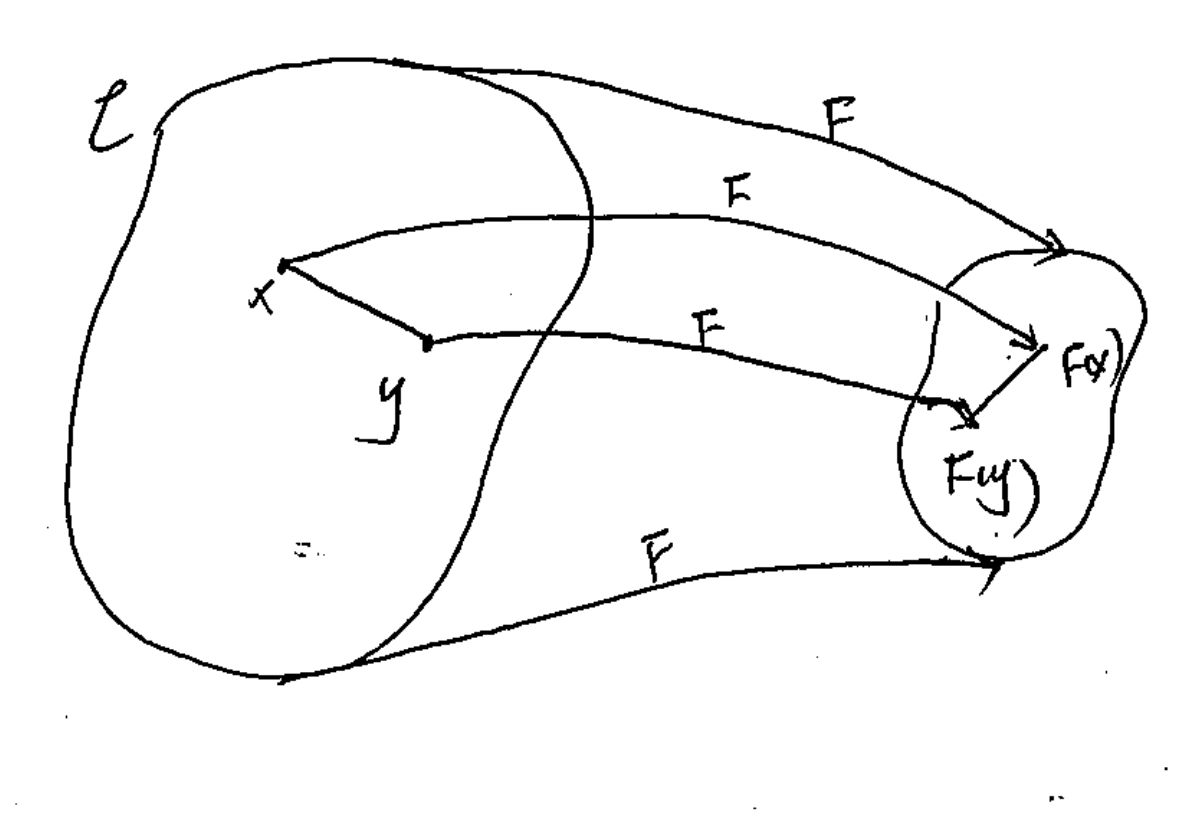
\includegraphics[width=1.8in,height=1.8in]{figures/ch08/figure1023_5.png}
	%\caption{This is an inserted JPG graphic} 
	%\label{fig:graph} 
\end{marginfigure}


\noindent 5) Norm balls are convex (recall that a norm is defined as $\Vert  x\Vert_p = (\sum^n_{i=1}\vert  x_i\vert^p)^{\frac{1}{p}}$ for $p\geq 1$).

\begin{marginfigure}
	\centering
	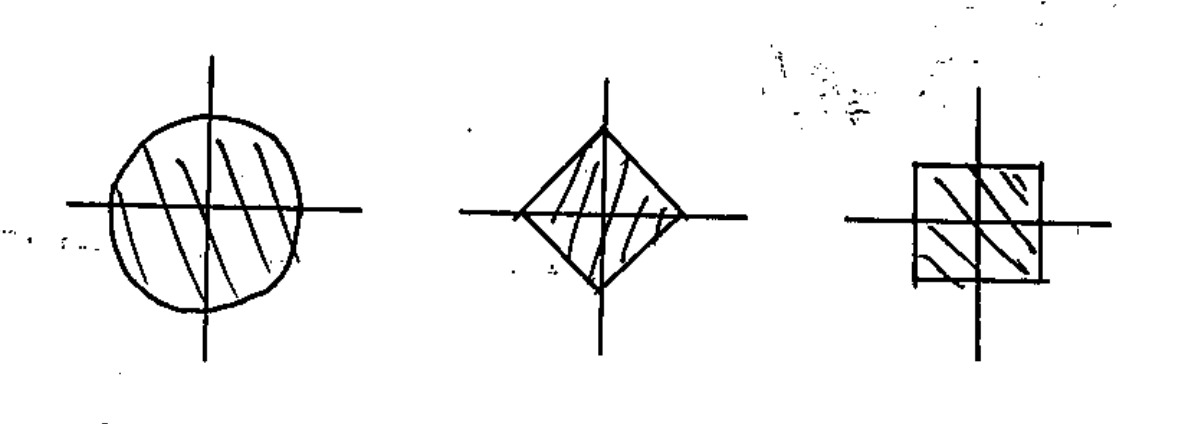
\includegraphics[width=1.8in,height=1.8in]{figures/ch08/figure1023_6.png}
	%\caption{This is an inserted JPG graphic} 
	%\label{fig:graph} 
\end{marginfigure}

\begin{proof}
	Take any two points $u,v$ s.t. $\Vert u\Vert \leq 1$, $\Vert v\Vert \leq 1$, by utilizing the triangular inequality and scaling property of a norm, we show that
	\begin{align*}
	\Vert \lambda u+(1-\lambda)v\Vert &\leq \Vert \lambda u\Vert + \Vert (1-\lambda)v\Vert\\
	&= \vert \lambda \vert \Vert  u\Vert + \vert (1-\lambda) \vert \Vert  v\Vert\\
	&= \lambda\Vert  u\Vert + (1-\lambda)\Vert  v\Vert\\
	&\leq \lambda 1 + (1-\lambda)1\\
	&= 1
	\end{align*}
\end{proof}

\begin{example}
The ellipsoids defined as
\begin{equation*}
\xi(x_c, P) =\{x|(x - x_c)^{\trans}P^{-1}(x - x_c) \leq 1 \}
\end{equation*}
is a convex set, where $P\in S^n_{++}$.

\begin{proof}
	First recall that $l_2$ norm ball is convex, and consider following affine map
	$$F(u) = P^{\frac{1}{2}}u + x_c$$
	Therefore the set $\{F(u) | \Vert u\Vert_2 \leq 1 \}$ is convex. We show that this set is equivalent to a ellipsoid,
\begin{align*}
\{F(u) | \Vert u\Vert^2_2 \leq 1 \} &= \{x|x = P^{\frac{1}{2}}u+x_c, \Vert u\Vert^2_2 \leq 1 \}\\
&= \{x|x - x_c = P^{\frac{1}{2}}u, \Vert u\Vert^2_2 \leq 1 \}\\
&= \{x|P^{-\frac{1}{2}}(x - x_c) =u, \Vert u\Vert^2_2 \leq 1 \}\\
&= \{x|\Vert P^{-\frac{1}{2}}(x - x_c)\Vert^2_2 \leq 1 \}\\
&= \{x|(x - x_c)^{\trans}P^{-1}(x - x_c) \leq 1 \}
\end{align*}
So the set $\xi(x_c, P) =\{x|(x - x_c)^{\trans}P^{-1}(x - x_c) \leq 1 \}$ is a convex set.

Also, remind that in previous QP chapter, we intersect these shapes with polyhedron to get the feasible set of QCQP.
\end{proof}
\end{example}

\begin{example}Consider the set
	$$\{x | \Vert Ax - b \Vert^2_2 \leq 1 \} = \{x | \Vert F(x) \Vert^2 \leq 1 \}$$
	where $F(x) = Ax - b$.

	This set is the pre-image(inverse image) of a convex set(norm ball is a convex set) under an affine function, and so it's convex.
\end{example}


%Above are notes for Oct23


%Below are notes for Oct30
%Consider an affine function $F(x) = Ax + b$, $A\in \reals^{m\times n}$, $b\in \reals^m$, $F:\reals^n \rightarrow \reals^m$
%
%Then:
%
%\begin{enumerate}
%	\item $\forall \mathcal{C}\subseteq \reals^n$ that are convex, the image of $\mathcal{C}$ under action of $F$ is a convex set in $\reals^m$:
%	
%	\begin{equation*}
%	F(\mathcal{C}) = \{F(x)\in \reals^m \vert x\in \mathcal{C} \}
%	\end{equation*}
%	
%	\item $\forall \mathcal{C}\subseteq \reals^m$ that are convex, the pre-image ("inverse image") of $\mathcal{C}$ under $F$: 
%	\begin{equation*}
%	F^{-1}(\mathcal{C}) = \{x| F(x)\in \mathcal{C} \}
%	\end{equation*}
%	is a convex set $\in \reals^n$
%\end{enumerate}
%
%Used (1) show:
%\begin{itemize}
%	\item all norm balls are convex sets.
%	
%	\item ellipsoids are convex sets.
%\end{itemize}
%
%\begin{example}
%	$\{x|\Vert Ax + b\Vert \leq 1 \}$ is a convex set$\rightarrow$ 
%	
%	Let $F(x) = Ax + b$(affine function)
%	
%	Let $\beta = \{x|\Vert x \Vert \leq 1 \}\in \reals^m$
%	
%	\begin{align*}
%	\{x|\Vert Ax+b\Vert\leq 1 \} &= \{x|\Vert F(x) \Vert\leq 1 \}\\
%	&= \{x|F(x) \leq \beta \}\\
%	&= F^{-1}(\beta)
%	\end{align*}
%\end{example}
%
%\vspace{0.5cm}

\vspace{0.4cm}
\subsection{Cones and generalized inequalities}
We introduce some important cones here and first recall the following definitions for set of symmetric matrices, set of PSD matrices and set of PD matrices,
\begin{align*}
S^n &= \{x\in \reals^{n\times n}\ s.t.\ x = x^{\trans} \}\\
S^n_+ &= \{x\in S^{n}\ s.t.\ v^{\trans}Xv \geq 0, \forall v\in \reals^n \}\\
S^n_{++} &= \{x\in S^{n}\ s.t.\ v^{\trans}Xv > 0 ,\forall v\in \reals^n\}
\end{align*}

Sets of PSD and PD matrices are two class of important cones, and recall the definition of cone: Set $\mathcal{C}$ is a cone if $\forall x\in \mathcal{C}$ and $\theta \in \reals_{+}$(i,e. $\theta \geq 0$), $\theta x\in \mathcal{C}$. In particular,  \\ 

\vspace{0.2cm}
\noindent 1) $S_+^n$ is a cone.

Since $\forall X \in S_+^n$ and $\forall \theta \geq 0$, we have
$$v^{\trans}(\theta X)v = \theta v^{\trans}Xv  > 0$$
We write:
\begin{align*}
X\in S^n_+ &\Leftrightarrow X\geq 0\\
X\in S^n_{++} &\Leftrightarrow X> 0
\end{align*}

\vspace{0.2cm}
\noindent 2) $S_+^n$ is a convex cone.

Let $A\in S^n_+$, $B\in S^n_+$, and consider the combination $\lambda A + (1-\lambda)B$ where $\lambda \in [0,1]$.

First note that $(\lambda A + (1-\lambda)B)^{\trans}= \lambda A^{\trans} + (1-\lambda)B^{\trans} = \lambda A + (1-\lambda)B \in S^n$, so this combination is still a symmetric matrix.

Secondly, we show that $v^{\trans}(\lambda A + (1-\lambda B))v =\lambda(v^{\trans}Av) + (1-\lambda)(v^{\trans}Bv)\geq 0$, so this combination is still a PSD matrix. 

Therefore, $S_+^n$ is convex and thus it is a convex cone.

\vspace{0.2cm}
\noindent 3) $S^n_{++}$ is also a convex cone. 

The proof follows the same as previous case (2) except we replace $\geq$ with $>$.



\vspace{0.3cm}
\textbf{Cones lead to "generalized" inequalities.}

We want to extend idea of orderings to $\reals^n$ (i.e., extend the comparison between two real numbers to two real vectors/matrices), and let's start with a "proper" cone $K\in \reals^n$. 

\begin{definition}[Proper cone]
A cone $K\in \reals^n$ is called a proper cone if it satisfies the following
\begin{itemize}
	\item $K$ is convex.
	\item $K$ is closed. 
	\item $K$ is solid, which means it has nonempty interior.
	\item $K$ is pointed, which means that it contains no line (or equivalently, $x \in K, -x\in K \Rightarrow x=0$).
\end{itemize}
\end{definition}


A proper cone $K$ can be used to define a generalized inequality $\leq_K$, says "less-than-or-equal to with respect to cone $K$".

Interpretation of $\leq_K$ and $< K$:
\begin{align*}
x\leq_K y &\Leftrightarrow 0\leq_K (y-x)\Leftrightarrow y - x \in K\\
x <_Ky &\Leftrightarrow y-x\in \text{int}(K)
\end{align*}
where the set int$(K)$ denotes the points in the interior of $K$.

\begin{marginfigure}
	\centering
	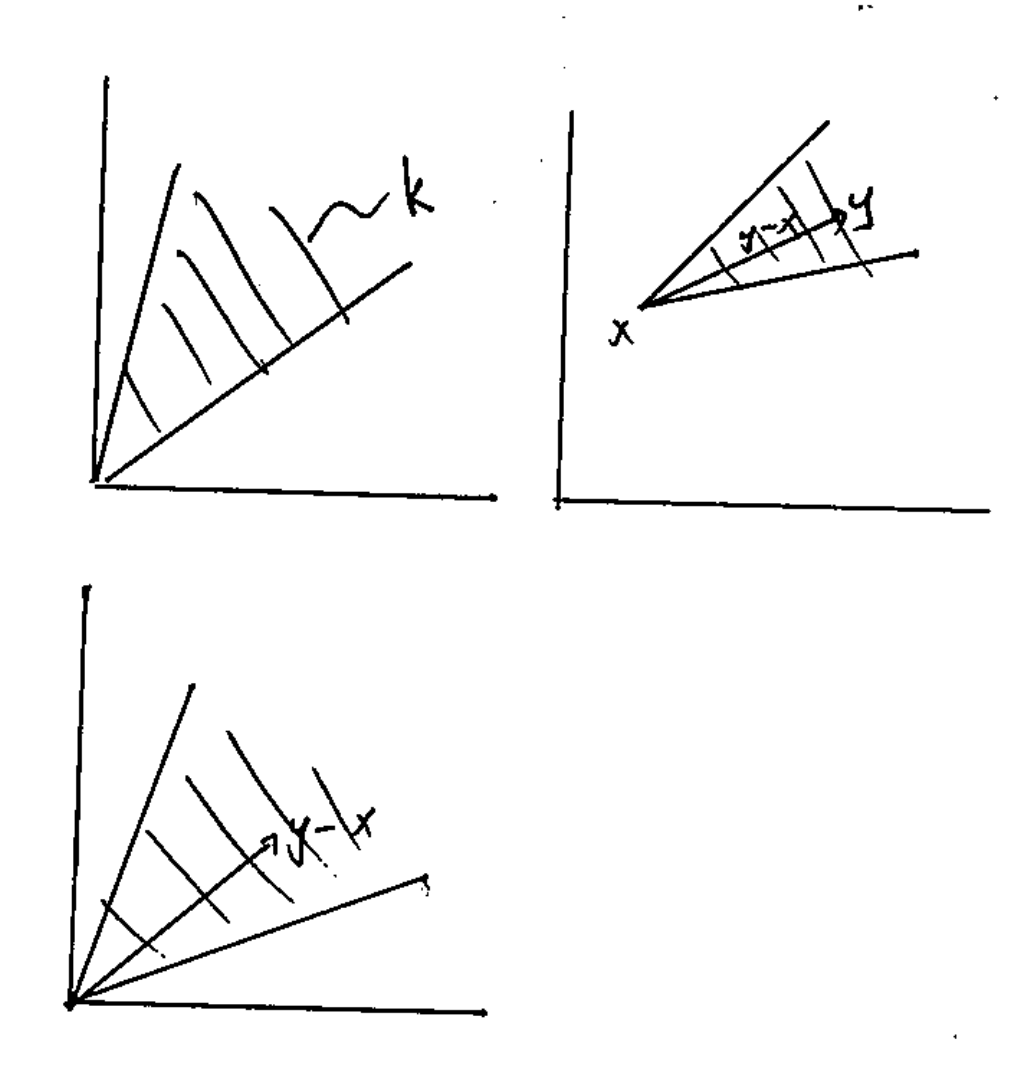
\includegraphics[width=1.8in,height=1.8in]{figures/ch08/figure1030_1.png}
	%\caption{This is an inserted JPG graphic} 
	%\label{fig:graph} 
\end{marginfigure}


\begin{example}
	Let a proper cone $k = S^n_+$, which denote the ordering of matrices, whose elements of vector space are in $S^n$. So,
	$$X\leq_k Y \Leftrightarrow 0\leq_k Y-X.$$
	Thus, $Y-X\in S^n_+$.
	
	$\rightarrow$ It true since that $v^{\trans}(Y-X)v \geq 0$, $\forall v\in \reals^n$
	
	$\rightarrow$ All eigenvalues are non-negative.
	
	Note: The interior of $S_+^n$ is $S^n_{++}$.
	
\end{example}

\vspace{0.3cm}
The following 2 generalized inequalities come up so often, so we assume that they are the default settings.
\begin{enumerate}
	\item If we compare 2 vectors $x,y\in \reals^n$, we write 
	$$x\leq  y\Leftrightarrow x\leq_{\reals^n_{+}}y \Leftrightarrow y-x\in \reals^n_{+}$$ 
	
	\item If we compare 2 symmetric matrices, we write:
	\begin{align*}
	x\leq y &\Leftrightarrow x\leq_{S_+^n} y\Leftrightarrow y - x\in S^n_{+}\\
	x< y &\Leftrightarrow y - x\in S^n_{++}
	\end{align*}
\end{enumerate}

\begin{example}
Consider the set $\{x\in \reals^n | x_1A_1 + x_2A_2 + ... + x_nA_n \leq B\}$, where $A_i\in S^m$, $B\in S^m$. The inequity here is called the "linear matrix inequality", and notice that $F(x) = B - \sum^n_{i=1}x_iA_i$ is an affine function of $x$. 

Hence,
\begin{align*}
\{x\in \reals^n | x_1A_1 + x_2A_2 +\cdots + x_nA_n \leq B\}
 &= \{x\in \reals^n | F(x)\geq 0\}\\
 &= \{x\in \reals^n | F(x)\in S^n_+ \}\\
 &=F^{-1}(S^n_+)
\end{align*}

So, it is a convex set, since the set is the pre-images of a convex set $S_+^n$ under an affine transform.
\end{example}

\vspace{0.5cm}
\textbf{Properties of Convex Sets:}

\begin{marginfigure}
	\centering
	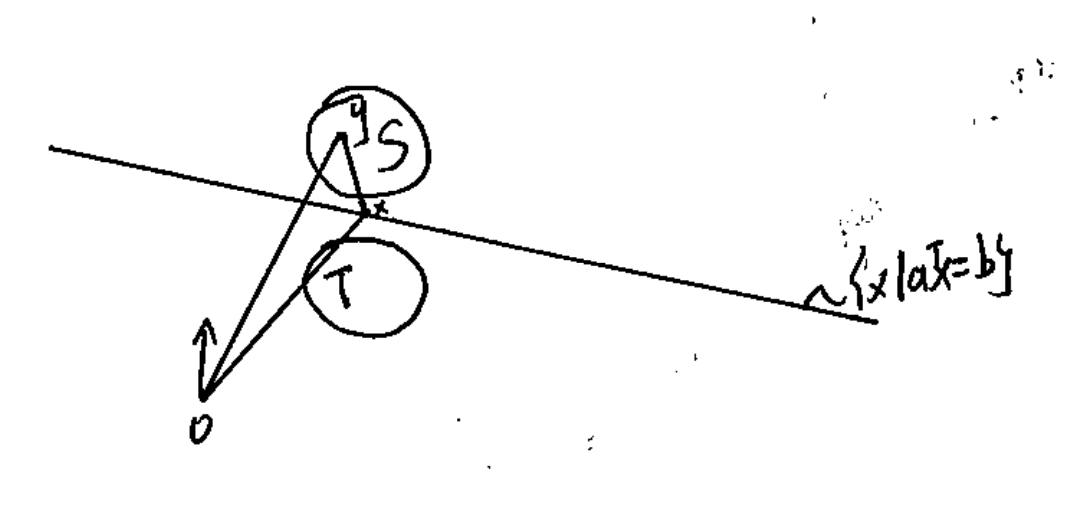
\includegraphics[width=1.8in,height=1.8in]{figures/ch08/figure1030_2.png}
	%\caption{This is an inserted JPG graphic} 
	%\label{fig:graph} 
\end{marginfigure}


\begin{enumerate}
	\item Separating hyperplane: 
	\begin{marginfigure}
		\centering
		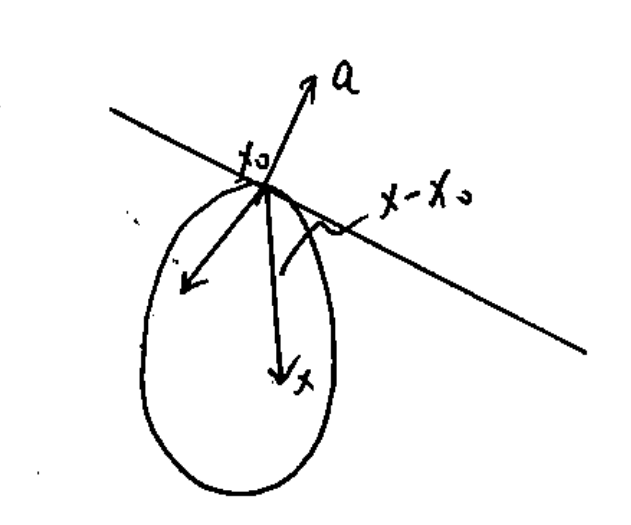
\includegraphics[width=1.8in,height=1.8in]{figures/ch08/figure1030_3.png}
		%\caption{This is an inserted JPG graphic} 
		%\label{fig:graph} 
	\end{marginfigure}
	
	\begin{marginfigure}
		\centering
		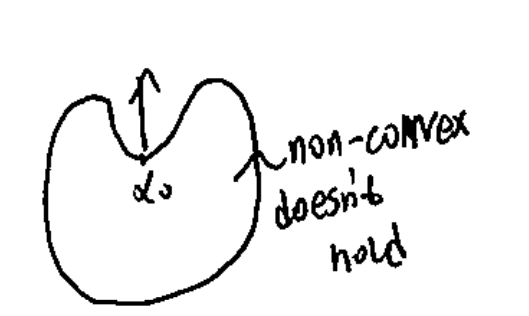
\includegraphics[width=1.8in,height=1.8in]{figures/ch08/figure1030_4.png}
		%\caption{This is an inserted JPG graphic} 
		%\label{fig:graph} 
	\end{marginfigure}
	
	\begin{marginfigure}
		\centering
		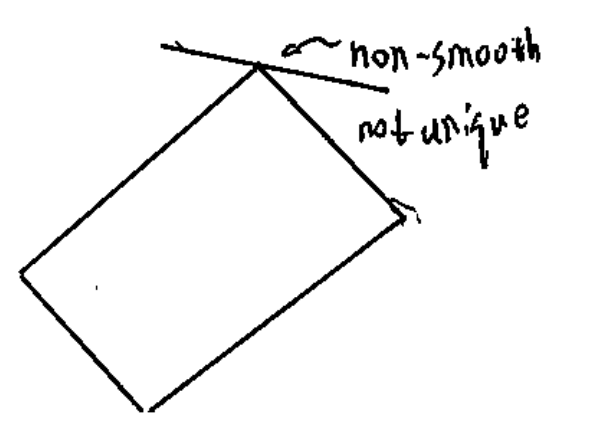
\includegraphics[width=1.8in,height=1.8in]{figures/ch08/figure1030_5.png}
		%\caption{This is an inserted JPG graphic} 
		%\label{fig:graph} 
	\end{marginfigure}
	If $S,T$ are convex sets in $\reals^n$ and disjoint, i.e, $S\cap T = \emptyset$, then there exists an $a \in \reals^n$ and $b\in \reals$ s.t.	
	\begin{align*}
	a^{\trans}y&\geq b, \forall x\in S\\
	a^{\trans}x &<b, \forall x\in T                              
	\end{align*}
	Hence,
	 $$a^{\trans}y - a^{\trans} x = a^{\trans}(y-x) \geq 0$$
	

	\item Supporting hyperplanes:


	If $S$ is a convex set, then $\forall x_0\in \delta \mathcal{S}$ (boundary of $S$) and $\forall x\in S$, $\exists a\in \reals^n$ such that 
	$$a^{\trans}x \leq a^{\trans}x_0\Leftrightarrow a^{\trans}(x - x_0)\leq 0$$

	
\end{enumerate}

\subsection{Convex Functions}
Let $F$ have a convex domain, then $F:\reals^n\rightarrow \reals$ is a convex function if $\forall x,y \in \text{dom} (F)$:
\begin{equation*}
F(\lambda x + (1-\lambda)y) \leq \lambda F(x) + (1-\lambda)F(y),\ \forall \lambda \in [0,1]
\end{equation*}
and $F$ is strictly convex if 
\begin{equation*}
F(\lambda x + (1-\lambda)y) < \lambda F(x) + (1-\lambda)F(y), \forall\ \lambda \in (0,1)
\end{equation*}

Note: $F$ is a "concave" function if $-F$ is convex.

\begin{marginfigure}
	\centering
	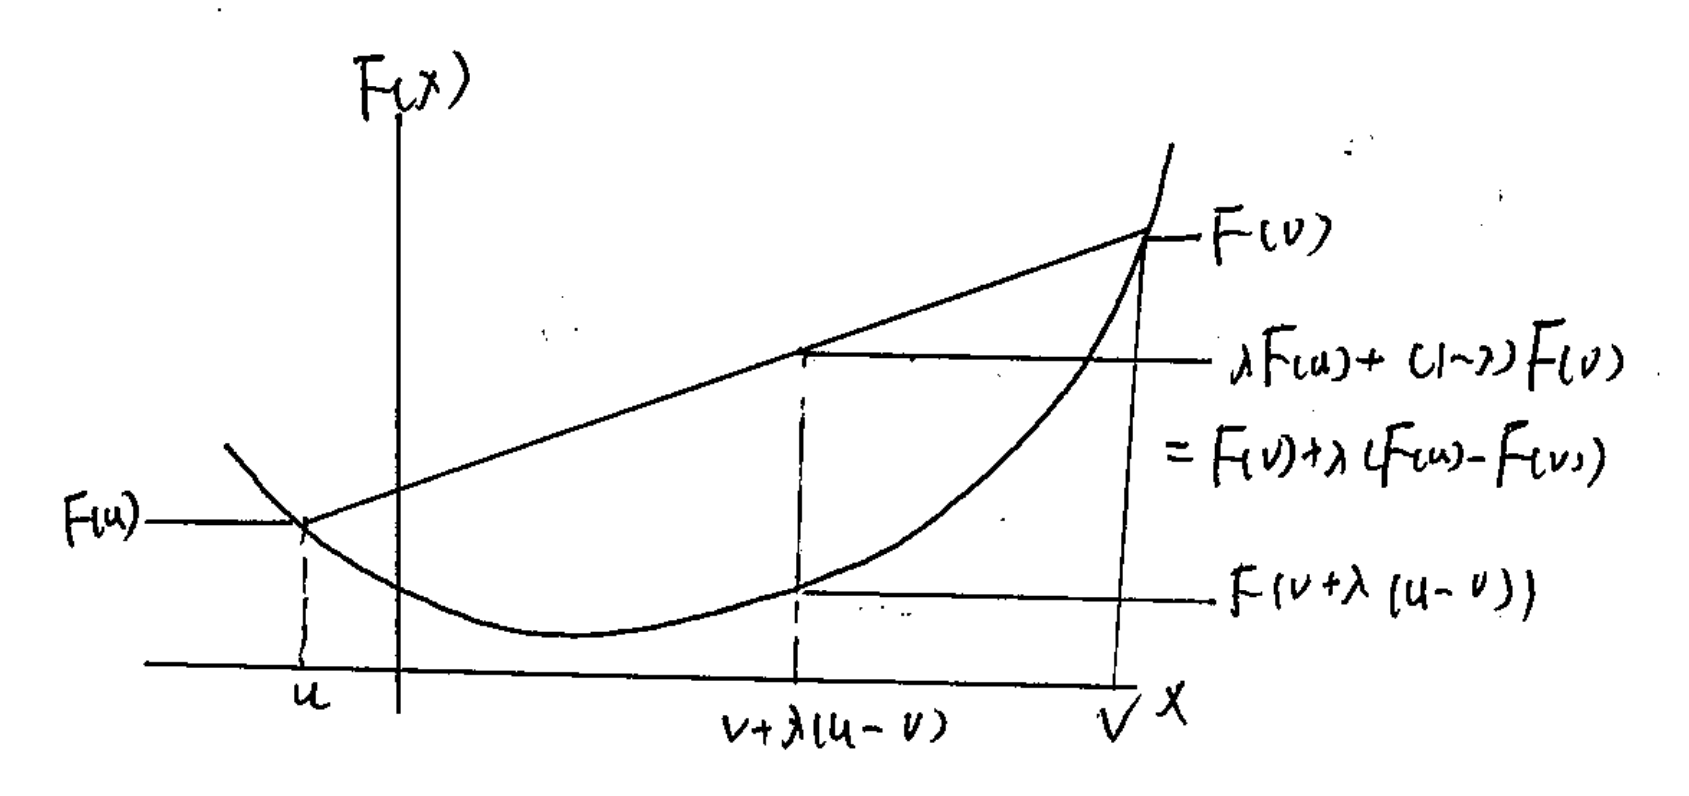
\includegraphics[width=1.5in,height=1.5in]{figures/ch08/figure1030_6.png}
	%\caption{This is an inserted JPG graphic} 
	%\label{fig:graph} 
\end{marginfigure}

Definition of convex:
	
\begin{marginfigure}
	\centering
	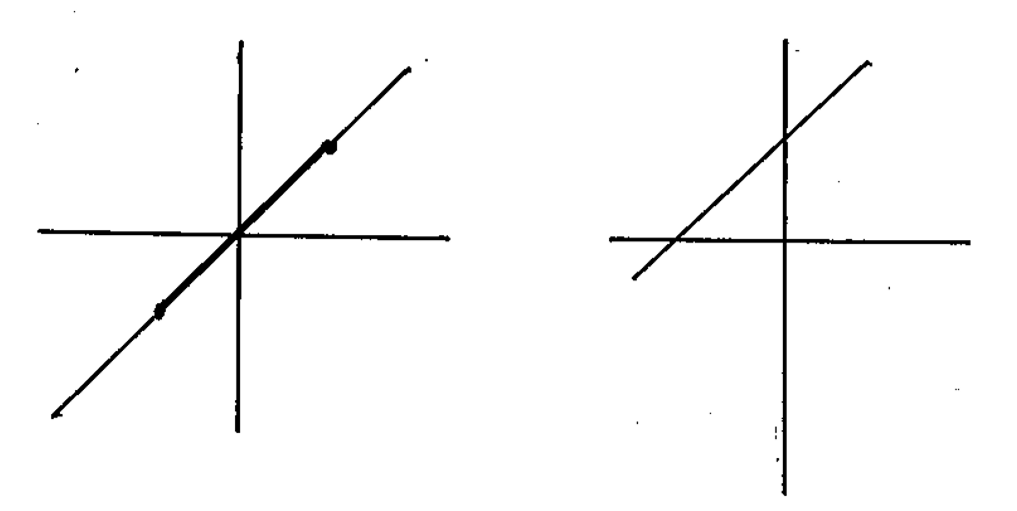
\includegraphics[width=1.5in,height=1.5in]{figures/ch08/figure1030_7.png}
	%\caption{This is an inserted JPG graphic} 
	%\label{fig:graph} 
\end{marginfigure}

\begin{marginfigure}
	\centering
	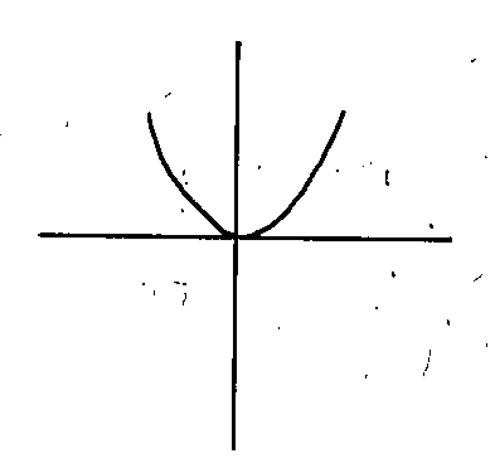
\includegraphics[width=1.5in,height=1.5in]{figures/ch08/figure1030_8.png}
	%\caption{This is an inserted JPG graphic} 
	%\label{fig:graph} 
\end{marginfigure}

\begin{marginfigure}
	\centering
	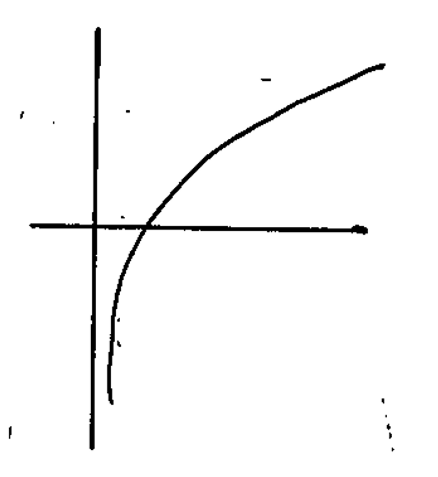
\includegraphics[width=1.5in,height=1.5in]{figures/ch08/figure1030_9.png}
	%\caption{This is an inserted JPG graphic} 
	%\label{fig:graph} 
\end{marginfigure}

\begin{marginfigure}
	\centering
	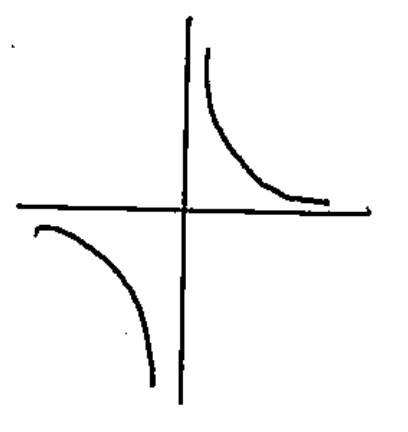
\includegraphics[width=1.5in,height=1.5in]{figures/ch08/figure1030_10.png}
	%\caption{This is an inserted JPG graphic} 
	%\label{fig:graph} 
\end{marginfigure}


\begin{equation*}
F(\lambda u + (1-\lambda)v) \leq \lambda F(u) + (1-\lambda)F(v)
\end{equation*}

And $F(\lambda u + (1-\lambda)v)$ can be written as $F(v + \lambda(u-v))$:

\begin{equation*}
F(\lambda u + (1-\lambda)v) \leq \lambda F(v) + \lambda(F(u)-F(v))
\end{equation*}

line segment connecting $(u,F(u))$ to $(v, F(v))$ always above bottom of bowl.


Sometimes define an "extended value" function

$$ \tilde{F}(x)=\left\{
\begin{array}{rcl}
F(x)       &      & \text{if } x\in \text{dom}(F)\\
\infty   &      & else
\end{array} \right. 
$$

\begin{example}[Examples of convex/concave functions]

Refer to the figures on r.h.s.

	(1) Linear function and affine functions are both convex and concave.
	
	(2) $F(x)=x^2$ is convex.
	
	(3) $F(x) = \log x$ with $\text{dom}\ F = \reals_{++}$ is a concave function.
	
	(4) The norm function $\Vert x\Vert$ is convex. 
	
	Since we have
	\begin{align*}
	\Vert \lambda x + (1-\lambda)y\Vert 
	&\leq \Vert \lambda x\Vert + \Vert(1-\lambda)y\Vert\\
	&=\lambda \Vert x \Vert + (1-\lambda)\Vert y \Vert
	\end{align*}
	
	(5) $F(x)=\frac{1}{x}$ is convex on $\reals_{++}$, and is concave on $\reals_{--}$.
	
\end{example}
	
\vspace{0.5cm}
\begin{definition}[Epigraph]
Recall the epigraph of a function is a set of points lying on or above its graph:
\begin{equation*}
\text{epi}\ F = \{(x,t)|t\geq F(x), x\in \text{dom}\ F, t\in\reals \}
\end{equation*}
\end{definition}

\begin{marginfigure}
	\centering
	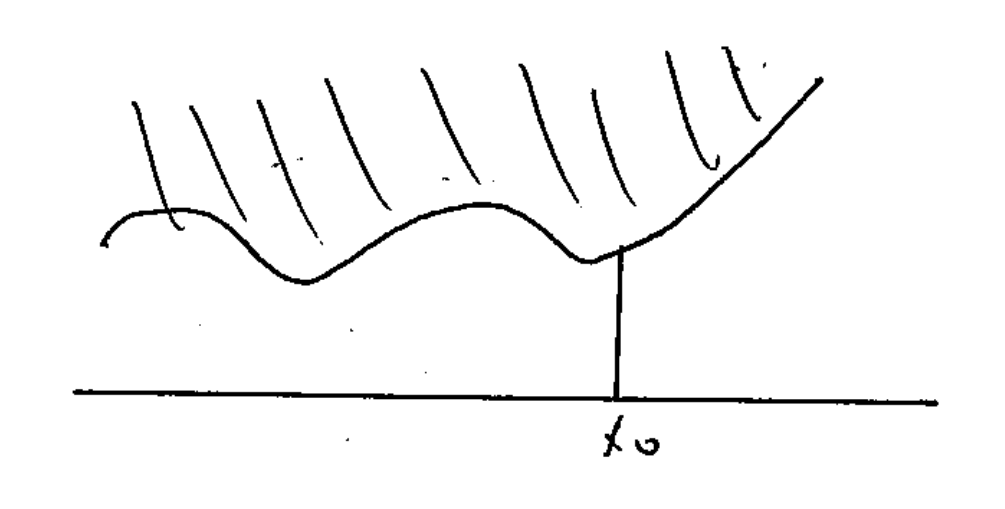
\includegraphics[width=1.8in,height=1.8in]{figures/ch08/figure1030_11.png}
	%\caption{This is an inserted JPG graphic} 
	%\label{fig:graph} 
\end{marginfigure}

\begin{definition}
	$F$ is a convex function iff $\text{epi}\ F$ is a convex set
\end{definition}

\begin{definition}[Sublevel sets] Recall that, the $\alpha$-sublevel set of a function $F$ is defined as
	$$\mathcal{C}(\alpha) = \{x|F(x)\leq \alpha, x\in \text{dom}F \}$$
	for $\alpha\in\reals$.
	\begin{marginfigure}
	\centering
	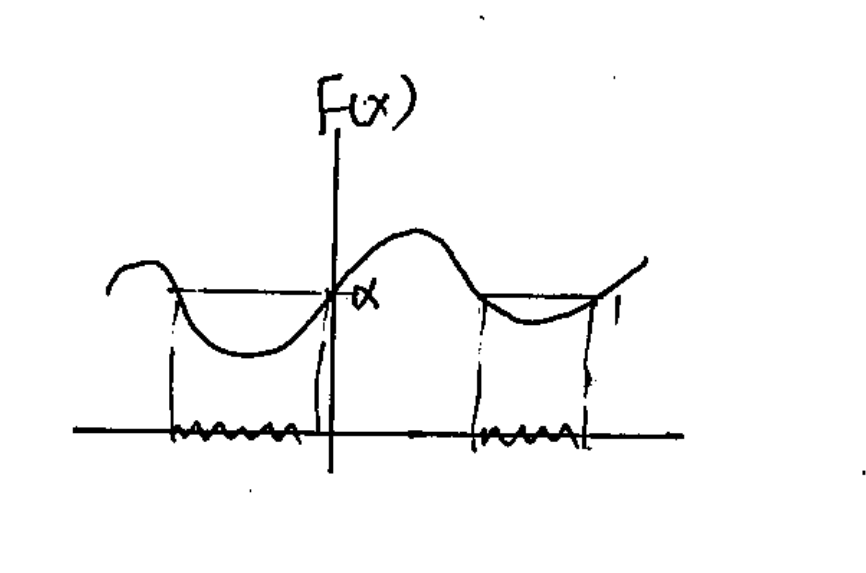
\includegraphics[width=1.8in,height=1.8in]{figures/ch08/figure1030_12.png}
	%\caption{This is an inserted JPG graphic} 
	%\label{fig:graph} 
	\end{marginfigure}
\end{definition}

\begin{theorem}
	If $F$ is convex, then its sub-level sets are all convex sets.
\end{theorem}
Note: The converse of this theorem is not true. If all sub-level sets of a function are convex sets, the function is "quasi-convex" but not necessarily convex.\\

\begin{marginfigure}
	\centering
	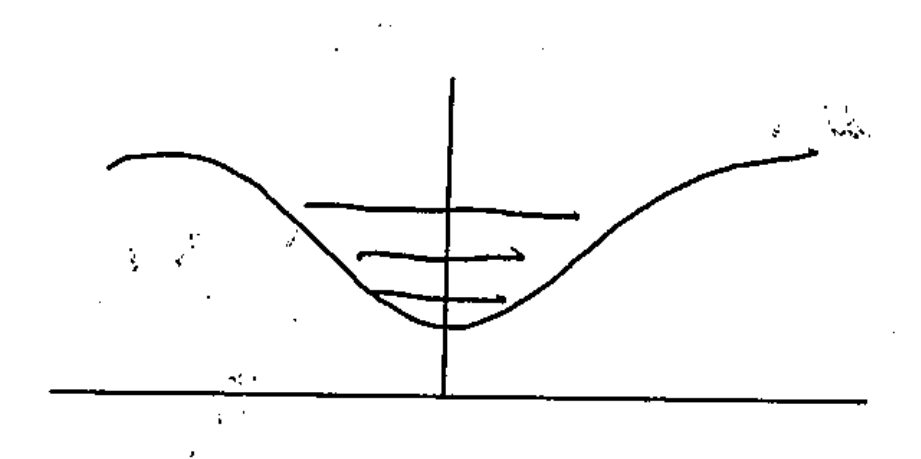
\includegraphics[width=1.8in,height=1.8in]{figures/ch08/figure1030_13.png}
	%\caption{This is an inserted JPG graphic} 
	%\label{fig:graph} 
\end{marginfigure}

\vspace{0.3cm}
\noindent \textbf{Three kinds of convex functions:}

1) Non-negative sums of convex functions are convex.

Let $F(x) =\sum^m_{i=1}a_iF_i(x)$, $F_i$ are convex function and $\text{dom}\ F = \cap^m_{i=1}\text{dom}\ F_i$. 

We show that such $F$ is a convex function,
\begin{align*}
F(\lambda x + (1-\lambda)y) 
&= \sum^m_{i=1}a_iF_i(\lambda x + (1-\lambda)y)\\
&\leq \sum^m_{i=1}a_i[\lambda F_i(x) + (1-\lambda)F_i(y)]\\
&= \lambda[\sum^m_{i=1}a_iF_i(\lambda)] + (1-\lambda)[\sum^m_{i=1}a_iF_i(y)]\\
&= \lambda[F(x)] + (1-\lambda)[F(y)]
\end{align*}

2) Convex functions of affine transformations of variables is still a convex function.

Let $g(x) =F(Ax + b)$, where $F(\cdot)$ is convex, and notice that $\text{dom}\ g = \{x|Ax + b \in\text{dom}\ F \}$. 

We show that function $g$ is convex in $x$,
\begin{align*}
g(\lambda x + (1-\lambda)y) &= F(A(\lambda x + (1-\lambda)y) + b)\\
&= F(\lambda(Ax + b) + (1-\lambda)(Ay+b))\\
&\leq \lambda F(Ax + b) + (1-\lambda)F(Ay+b)\\
&= \lambda g(x) + (1-\lambda)g(y)
\end{align*}


3) The max of a pair of convex functions is a convex function:
\begin{equation*}
g(x) = \max\{F_1(x), F_2(x) \}
\end{equation*}


\begin{marginfigure}
	\centering
	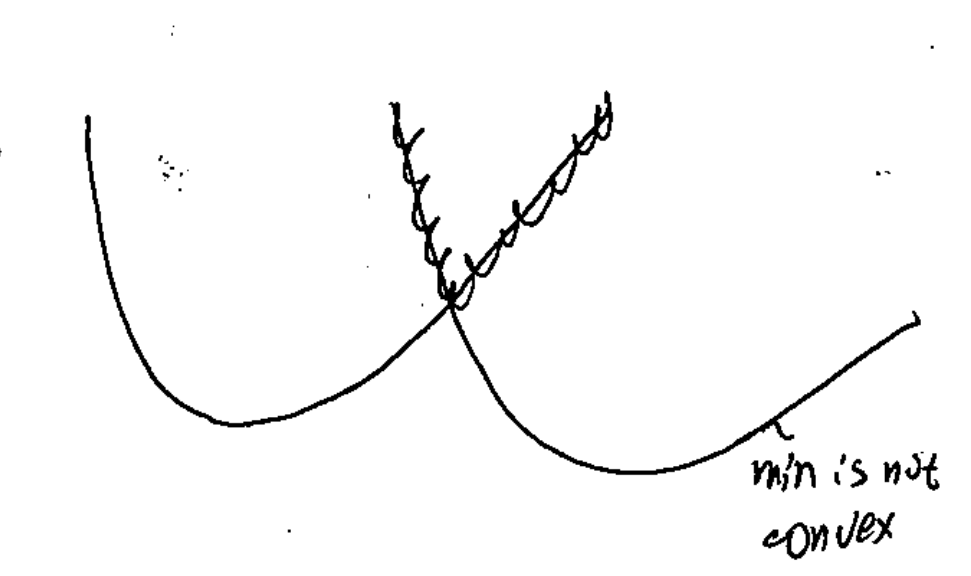
\includegraphics[width=1.8in,height=1.8in]{figures/ch08/figure1030_14.png}
	%\caption{This is an inserted JPG graphic} 
	%\label{fig:graph} 
\end{marginfigure}
%Above are notes for Oct30




%Below are notes for Nov 4
\subsection{More examples}
Let's consider following three kinds of functions we have mentioned above,
\begin{align*}
F(x) &=\sum\alpha_iF_i(x), \forall \alpha_i\geq 0\\
g(x) &= F(Ax + b)\\
g(x) &=\max\{F_1(x), F_2(x) \}
\end{align*}

\begin{example} Consider the function 
\begin{align*}
F(x) 
&= \sum^{n}_{i=1}log(b_i - a_i^{\trans}x)^{-1}\\
&=\sum^n_{i=1}-log(b_i - a_i^{\trans}x)
\end{align*}
where $x \in \reals^n$, $a_i\in \reals^n$, $b_i\in \reals$.

1) Note: $-log(\cdot)$ is a convex function, and 
$$\text{dom}-log(\cdot) = R_{++}$$
$$\text{dom}F = \{x|b_i - a_i^{\trans}x >0, \forall i\in [m] \} =\{x|b_i - a_i^{\trans}x \in \reals_{++}, \forall i\in [m]\}$$ 

So, the domain of this function is the inverse image of $\reals_{++}$(a convex set) under an affine transformation, and therefore it is a convex set. 

2) Each function is a convex function of an affine transformation of $x$, therefore the sum of these functions is still a convex function.
\end{example}

\begin{example}
\begin{marginfigure}
	\centering
	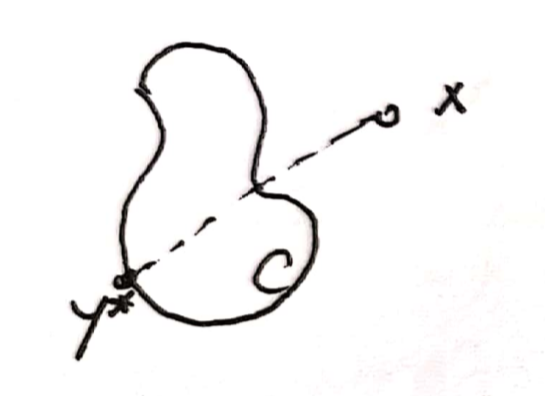
\includegraphics[width=1.8in,height=1.8in]{figures/ch08/figure1104_1.png}
	%\caption{This is an inserted JPG graphic} 
	%\label{fig:graph} 
\end{marginfigure}

\begin{equation*}
F(x) = \sup_{y\in \mathcal{C}}\Vert y-x\Vert
\end{equation*}

Note that $\mathcal{C}$ is not necessarily to be a convex set. 

\begin{enumerate}
	\item Function $y-x$ is an affine function w.r.t $x$ and therefore it is a convex function of $x$.
	
	\item $\Vert\cdot\Vert$ is a norm function, so it is a convex function of its argument. 
	
	\item $F(x) = \sup_{y\in \mathcal{C}}\Vert y-x\Vert$, $y\in \mathcal{C}$ is the basic max of a bunch of convex functions, each indexed by a $y\in \mathcal{C}$
\end{enumerate}
\end{example}



\begin{example}
\begin{equation*}
F(x) =\inf_{y\in \mathcal{C}}\Vert y-x\Vert
\end{equation*}

$\rightarrow$ Generally this function is NOT convex in $x$.

$\rightarrow$ If the set $\mathcal{C}$ is a convex set, then this function is convex in $x$. 
\end{example}




\begin{theorem}[Projection theorem]
 If $h(x, y)$ is convex in $(x,y)$, then $F(x) = \inf_yh(x,y)$ is convex in $x$.
\end{theorem}

\begin{marginfigure}
	\centering
	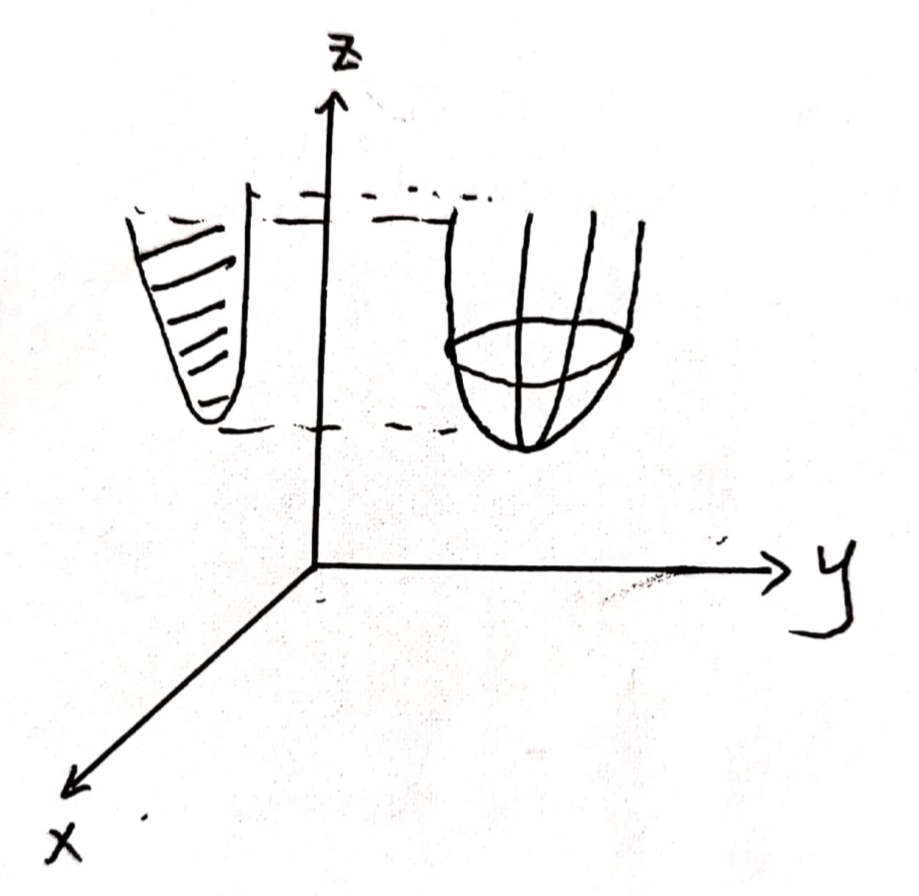
\includegraphics[width=1.8in,height=1.8in]{figures/ch08/figure1104_2.png}
	%\caption{This is an inserted JPG graphic} 
	%\label{fig:graph} 
\end{marginfigure}

Idea: Shine light along $y$-axis, and get the shadow on $x-z$ plane, which is an epi $F$ and it is a convex set. 

\begin{proof}
	Since $h(x,y)$ is convex in 
	$\begin{bmatrix}
	x\\
	y
	\end{bmatrix}
	\in \text{dom}\ h$, the epigraph of $h$ is given by 
	\begin{equation*}
	\text{epi}\ h = \{(x,y,t)|t\geq h(x,y), \begin{bmatrix}
	x\\
	y
	\end{bmatrix}\in \text{dom}\ h \}
	\end{equation*}
	That's the black bowl in the graph. 
	
	Now consider:
	\begin{equation*}
	F(x) = \inf_{y:
		\begin{bmatrix}
		x&y
		\end{bmatrix}^{\trans}
		\in \text{dom}\ h}
	\ h(x,y)
	\end{equation*}
	So the domain is given by
	\begin{align*}
	\text{dom}\ F &= \{x|\exists\ y\ s.t. (x,y)\in \text{dom}\ h \}\\
	&= \{\begin{bmatrix}
	1&0
	\end{bmatrix}
	\begin{bmatrix}
	x\\
	y
	\end{bmatrix} 
	|
	\begin{bmatrix}
	x\\
	y
	\end{bmatrix}\in \text{dom}\ h \}
	\end{align*}
	
	Note that this domain is an affine map of all points in a convex set, and therefore \text{dom} F is a convex set.
	
	Consider the epigraph of $F$,
\begin{align*}
\text{epi}\ F 
&= \{(x,t)|t\geq \inf_{y:
	\begin{bmatrix}
	x&y
	\end{bmatrix}^{\trans}
}
\in \text{dom}\ h, x\in \text{dom}\ F \}\\
&= \{
\begin{bmatrix}
1&0&1
\end{bmatrix}
\begin{bmatrix}
x\\
y\\
t
\end{bmatrix}
\vert t\geq h(x,y), 
\begin{bmatrix}
x\\
y
\end{bmatrix}\in \text{dom}\ h \}
\end{align*}

So this set is a convex set, and since it is the epigraph of $F$, $F$ must be a convex function. 

\end{proof}


\begin{example}
The function
\begin{equation*}
F(x) = \inf_{y\in\mathcal{C}}\Vert x-y\Vert
\end{equation*}
is a convex function if $\mathcal{C}$ is a convex set. 

\begin{enumerate}
	\item $x-y$ is affine in $x$
	
	\item $\Vert\cdot\Vert$ is a convex function for all norms.
	
	\item Apply projection theorem where $\text{dom}\ h = \{\begin{bmatrix}
	x\\
	y
	\end{bmatrix}\vert x\in \reals^n, y\in \mathcal{C} \}$ is a convex set and $x$ is unconstrained. 
\end{enumerate}
\end{example}


\subsection{Characterizing Convexity by Restricting to a Line}

\begin{theorem} $F: \reals^n \rightarrow \reals$ is convex if and only if $g:\reals \rightarrow \reals$,
	$$g(t) =F(x_0 + tv), \text{dom}\ g = \{t| x_0 + tv \in \text{dom}\ F\}$$
	is convex for any $x_0\in\text{dom}\ F$, $v\in\reals^{n}$.
\end{theorem}
\begin{itemize}
	\item $g(t)$ is function restricted to a line/slice
	
	\item If all possible slices convex then so is $F$.
\end{itemize}

Note: need $x_0+tv\in \text{dom}\ F$, also note $\text{dom}\ F$ is a convex set. 

\begin{equation*}
g(t) = g_{x_0, v}(t) = F(x_0+tv)
\end{equation*}

\begin{equation*}
\text{dom}(g_{x_0, v}) = \{t|x_0+tv \in \text{dom}F \}
\end{equation*}

Therefore $\text{dom}(g_{x_0, v})$ is convex set for all $x_0, v$.

\begin{proof}
First, we show that, if $F$ is convex then $g$ is convex. 
\begin{align*}
\forall t_1, t_2&\in \text{dom}\ g, \lambda\in [0,1]\\
g(\lambda t_1 +(1-\lambda)t_2) &= F(x_0+[\lambda t_1+(1-\lambda)t_2]v)\\
&= F(\lambda[x_0 +t, v]+(1-\lambda)[x_0+t_2v])\\
&\leq \lambda F(x_0+t_1 v)+(1-\lambda)F(x_0+t_2v)\\
&=\lambda g(t_1) + (1-\lambda)g(t_2)
\end{align*}

Second, we show that if $g$ is convex in $t$, $\forall(x_0, v)$, then $F$ is convex. 

Pick arbitrary $x,y\in \text{dom}\ F$, let $x_0 =x$, $v=(y-x)$, consider $g_{x_0, v}(t)$ for $t\in[0,1]$:
\begin{align*}
g_{x_0, v}(t) &= F(x_0+tv)\\
&= F(x+t(y-x))\\
&= F((1-t)x+ty)
\end{align*}
Since $g_{x_0, v}$ is convex in $t$, so $F$ is convex in $t$. ($t$ plays role of $\lambda$)

\end{proof}




\begin{example}
\begin{equation*}
F(x) =\log\det (x^{-1})
\end{equation*}
Note:

(1) $\text{dom}\ F = S^n_{++}$ $\Leftrightarrow$ PD matrices.

(2) $S^n_{++} \subset S^n \leftarrow$ vector space of $n\times n$ symmetric matrices. 

To show this function $F$ is a convex function, we will show it is convex for all "lines".

The "line" in $S^n$ is $x_0 + tH$, where $x_0$ is a symmetric PD matrix, $t\in \reals$ and $H$ is symmetric matrix in $S^n$. So $x_0 + tH$ is a family of symmetric matrices.

\begin{marginfigure}
	\centering
	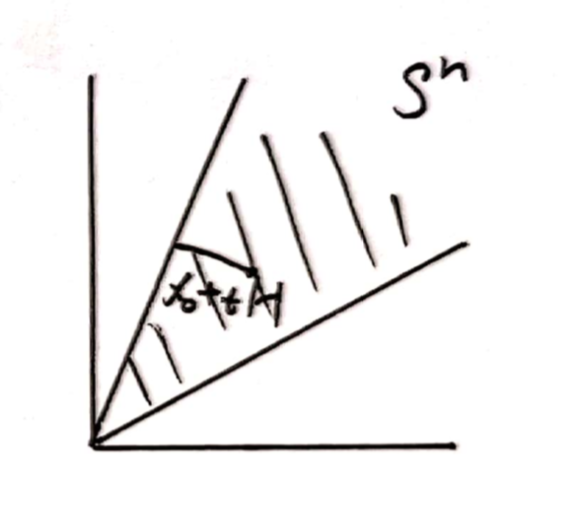
\includegraphics[width=1.8in,height=1.8in]{figures/ch08/figure1104_3.png}
	%\caption{This is an inserted JPG graphic} 
	%\label{fig:graph} 
\end{marginfigure}
\end{example}

Notice that $x_0\in S^n_{++}$, so $x_0^{-1}$exists and also $x_0^{\frac{1}{2}}$ exists. 
\begin{align*}
g(t) 
&= \log\det (x_0+tH)^{-1}\\
&= \log\det [(x_0^{\frac{1}{2}}x_0^{\frac{1}{2}}+tx_0^{\frac{1}{2}}x_0^{-\frac{1}{2}}+Hx_0^{-\frac{1}{2}}x_0^{\frac{1}{2}})^{-1}]\\
&= \log\det [x_0^{-\frac{1}{2}}(I+tx_0^{-\frac{1}{2}}Hx_0^{-\frac{1}{2}})^{-1}x_0^{-\frac{1}{2}}]\\
&= \log\det x_0^{-1} + \log\det[(I+tx_0^{-\frac{1}{2}}Hx_0^{-\frac{1}{2}})^{-1}]\\
&= \log\det x_0^{-1}+\log(\det(I+tM)^{-1})\\
&= \log\det x_0^{-1}+\log[\prod^n_{i=1}(1+t\lambda_i)^{-1}]\\
&= \log\det x_0^{-1} - \sum_{i=1}^n\log(1+t\lambda_i)
\end{align*}
In above inequalities we have utilized the property that $\det(AB) = \det(A)\cdot\det(B)$ and the determinant of a matrix equals to the product of its eigenvalues. 

Also, notice that
$$(I+tM)v = v+t\lambda v = (1+t\lambda)v$$
so the eigenvalues of $(I+tM)$ are $1+t\lambda_i$.\\

Note:
\begin{enumerate}
	\item $1+t\lambda_i$ is an affine map in $t$.
	
	\item Function $-log(\cdot)$ is convex.
	
	\item Combine above results, since it is a sum of convex functions, $g(t)$ is convex in $t$ (and thus $F(x)$ is convex in $x$).
\end{enumerate}


%Above are notes for Nov 4



\vspace{0.5cm}
\begin{example}
Consider the function of finding the max eigenvalue,
$$F(X) = \lambda_{\max}(X)$$
where $\text{dom}\ F = S^n$, and this function $F$ is convex.

We illustrate this fact by two parts.

(a) First, we have
$$\lambda_{\max}(X) = \max_{v:\Vert v\Vert = 1}v^{\trans}Xv$$
By eigen-decomposition of symmetric matrices,
\begin{align*}
v^{\trans}Xv 
&= v^{\trans}Q\Lambda Q^{\trans}v \\
&= \tilde{v}^{\trans}\Lambda \tilde{v}\\
&= \sum^n_{i=1}(\tilde{v}_i)^2\lambda_i \\
&\leq \lambda_{max}(X)
\end{align*}

(b) Express $x$ as following
\begin{equation*}
v^{\trans}(\alpha X_1 + \beta X_2)v = \alpha v^{\trans}X_1v + \beta v^{\trans}X_2v
\end{equation*}

So $v^{\trans}Xv$ is linear in $X$, and therefore $F(X)$ is the $\max$ of a bunch of functions that are linear in $X$, and thus it is convex.
\end{example}

\vspace{0.3cm}
\noindent\textbf{Two more examples}
\begin{enumerate}
	\item $F(x) = \sigma_{\max} (X)$ is convex on $\text{dom}\ F =\reals^{n\times m}$.
	
	\item $F(x) = (\det X)^{\frac{1}{n}}$, is concave on $\text{dom}\ F = S^n_{++}.$
\end{enumerate}

\vspace{0.5cm}
\subsection{"First-order" condition}

\begin{theorem}
	A differentiable function $F$ (i.e., $\text{dom}\ F$ is open and gradients exist everywhere in domain F) is convex if and only if $\forall x,y\in \text{dom}\ F$:
	\begin{equation*}
	F(y)\geq F(x) + \nabla F(x)^{\trans}(y-x) \qquad (*)
	\end{equation*}
	and is strictly convex if $(*)$ is a strict inequality for all $x\neq y$.
\end{theorem}
	\begin{marginfigure}
	\centering
	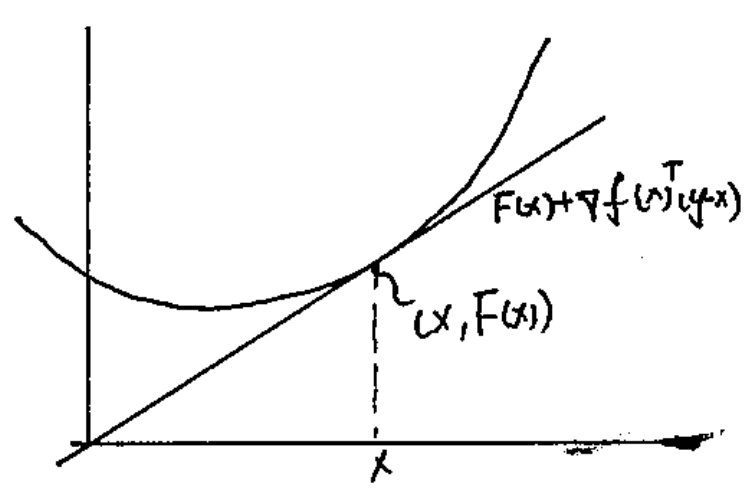
\includegraphics[width=1.8in,height=1.8in]{figures/ch08/figure1106_1.png}
	%\caption{This is an inserted JPG graphic} 
	%\label{fig:graph} 
	\end{marginfigure}
	Note that:
	
	(1) The affine function of $y$ given by $F(x) + \nabla F(x)^{\trans}(y-x)$ the First-order Taylor approximation, and the inequality above states that this approximation is an global underrestimator of $F$.
	
	(2) There is a tangent plane that is a supporting hyperplane of epi $F$.

\begin{proof}
First, assume $F$ is convex, and we show that $(*)$ holds. 

Take any $(x,y)\in \text{dom}\ F$, and by definition of convex function,
$$F((1-\lambda)x+\lambda y) \leq (1-\lambda)F(x) + \lambda F(y)$$

Rearrange yields
$$\frac{F(x+\lambda(y-x)) - F(x)}{\lambda} \leq F(y) - F(x)$$

Let $\lambda \rightarrow 0$ and observe that
$$lim_{\lambda\rightarrow 0} \frac{F(x+\lambda(y-x)) - F(x)}{\lambda} = \nabla F(x)^{\trans}(y-x)$$

Therefore,
$$\nabla F(x)^{\trans}(y-x)\leq F(y) - F(x)$$
Hence, the inequality $(*)$ holds (You can also do above procedure in 1-dimension, try it by yourself).


Secondly, we assume $(*)$ holds and show that $F$ is convex.

Take any $(x,y)\in \text{dom}\ F$, then $\forall \lambda\in[0,1]$, $z= \lambda x + (1-\lambda)y \in \text{dom}\ F$ since $\text{dom}\ F$ is convex.

Using $(*)$ for 2 times we get:
\begin{align*}
F(x) &\geq F(z) + \nabla F(x)^{\trans}(x-z)\\
F(y) &\geq F(z) + \nabla F(x)^{\trans}(y-z)
\end{align*} 

Compute
\begin{align*}
\lambda F(x)+(1-\lambda)F(y) &\geq F(z) + \nabla F(z)^{\trans}[\lambda (x-z)+(1-\lambda)(y-z)]\\
&= F(z) + \nabla F(z)^{\trans}[\lambda x - \lambda z + y - z - \lambda y +\lambda z]\\
&= F(z) + \nabla F(z)^{\trans}[\lambda x + (1-\lambda)y - z]\\
&= F(z) + \nabla F(z)^{\trans}[z - z]\\
&= F(z)\\
&= F(\lambda x + (1-\lambda )y)
\end{align*}

Therefore, the function $F$ is convex given that the inequality $(*)$ holds.
\end{proof}

\vspace{0.3cm}
\noindent\textbf{Connect $1$-st order condition with $\text{epi}\ F$}

Recall that $(x,t)\in \text{epi}\ F$ if $t\geq F(x)$, and the $1$-st order condition: $\forall x,y \in \text{dom}\ F$, $F(y)\geq F(x) + \nabla F(x)^{\trans}(y-x)$.

\begin{marginfigure}
	\centering
	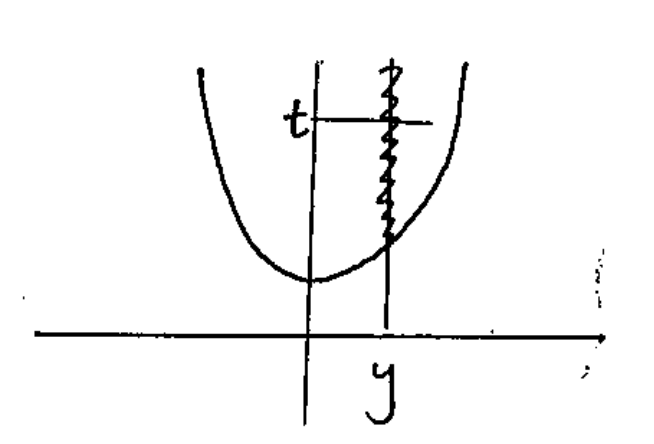
\includegraphics[width=1.8in,height=1.8in]{figures/ch08/figure1106_2.png}
	%\caption{This is an inserted JPG graphic} 
	%\label{fig:graph} 
\end{marginfigure}

Consider $\forall (y,t)\in \text{epi}\ F$:
\begin{align*}
t 
&\geq F(y) \geq F(x) + \nabla F(x)^{\trans}(y-x)\\
\Leftrightarrow 0 &\geq F(x) - t + \nabla F(x)^{\trans}(y-x)\\
&= 
\begin{bmatrix}
\nabla F(x)^{\trans} & -1
\end{bmatrix}
\begin{bmatrix}
y-x\\
t -F(x)
\end{bmatrix}\\
&= 
\begin{bmatrix}
\nabla F(x)^{\trans}  & -1
\end{bmatrix}
\begin{bmatrix}
y\\
t
\end{bmatrix} + (-\nabla F(x)^{\trans}x + F(x))
\end{align*}

\begin{marginfigure}
	\centering
	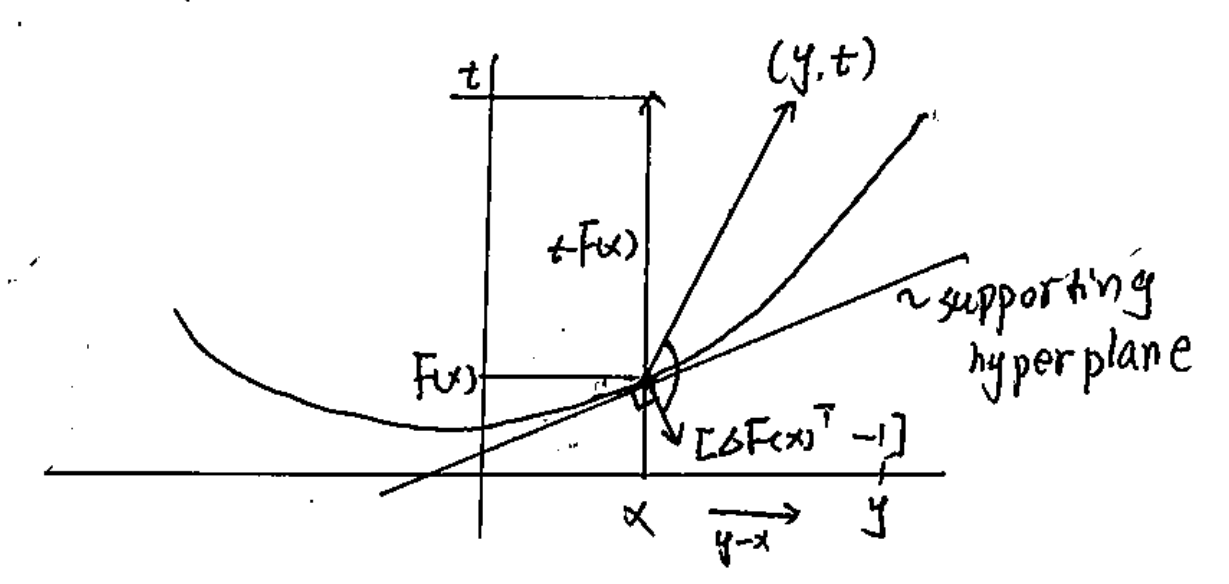
\includegraphics[width=1.8in,height=1.8in]{figures/ch08/figure1106_3.png}
	%\caption{This is an inserted JPG graphic} 
	%\label{fig:graph} 
\end{marginfigure}

\subsection{"Second-order" condition}

\begin{theorem}
	If $F$ is everywhere twice differentiable, then $F$ is convex if and only if its Hessian $\nabla^2F(x)\geq 0$ (i.e., PSD) for all $x\in \text{dom}\ F$.
\end{theorem}

\begin{proof}

Similarly, we prove this theorem in two steps.

Firstly, assume $F$ convex, and we show that $\nabla^2F(x)\geq 0$.

Let $x_0 \in \text{dom}\ F$(any point), $v\in \reals^n$(a direction), then $z = x_0 + \lambda v$ is in $\text{dom}\ F$ if $\lambda > 0$ sufficiently small. 

By Taylor approximation, 
$$F(z) = F(x_0) + \nabla F(x_0)^{\trans}(\lambda v) + \frac{1}{2}(\lambda_v)^{\trans}\nabla^2F(x_0)\lambda v + O(\lambda^3)$$

Rearrange yields 
$$\frac{1}{2}\lambda^2v^{\trans}\nabla^2F(x_0)v+O(\lambda^3) = F(z) - F(x_0) - \nabla F(x_0)^{\trans}(\lambda v)$$

The right-hand side is $\geq 0$ by first-order-convexity result.

Continuing, divide through by $\lambda^2$ to get:
$$\frac{1}{2}v^{\trans}\nabla^2F(x_0)v + \frac{O(\lambda^3)}{\lambda^2} \geq 0$$

In above equation, $O(\lambda^3)$ means this is $\leq M\lambda^3$ (Big-O notation), so $\frac{O(\lambda^3)}{\lambda^2} \leq M\lambda$.

Letting $\lambda\rightarrow 0$, we get 
$$\frac{1}{2}v^{\trans}\nabla^2F(x_0)v\geq 0$$
So $\nabla^2F(x_0)$ is PSD for all $x_0 \in \text{dom}f$, since $v\in \reals^n$ can be chosen arbitrarily.


\vspace{0.3cm}
Secondly, assume $\nabla^2F(x_0)\geq 0, \forall x_0\in \text{dom}\ F$, and we show that $F$ is convex.

Apply Taylor approximation with remainder $\forall x,y\in \text{dom}\ F$, 
$$F(y) =F(x) + \nabla F(x)^{\trans}(y-x) + \frac{1}{2}(y-x)^{\trans}\nabla^2F(z)(y-x)$$
where Hessian is evaluated at some $z$ between $x$ and $y$(Mean value theorem).

Since $\nabla^2F(z)\geq 0$, we have
$$F(y) \geq F(x) + \nabla F(x)^{\trans} (y-x)$$
Then we could go back to $1^{st}-$order-condition, which is true for $\forall x,y$. So $F$ must be convex. 
\end{proof}



Here we can give some examples:

\begin{enumerate}
	\item $F(x) = x^2$, $\text{dom}\ F = \reals$, $F''(x) = 2 > 0$, $\forall x\in \reals$, so $F$ is strictly convex.
	
	\item $F(x) = x^3$, $\text{dom}\ F = \reals$, $F'(x) = 3x^2$, $F''(x) = 6x$, so if we restrict the domain as $\text{dom}\ F = \reals_+$ then $F$ is convex.
	
	\item $F(x) = x^{\alpha}$, $\text{dom}\ F = \reals_+$, $F''(x) = \alpha(\alpha - 1)x^{\alpha - 2}$, where $\alpha(\alpha - 1) > 0$ if $\alpha > 1$ or $\alpha < 0$ and $\alpha(\alpha - 1) < 0$ if $0<\alpha < 1$. $x^{\alpha - 2}\geq 0$ since $\text{dom}\ F = \reals_+$.
	
	\begin{marginfigure}
	\centering
	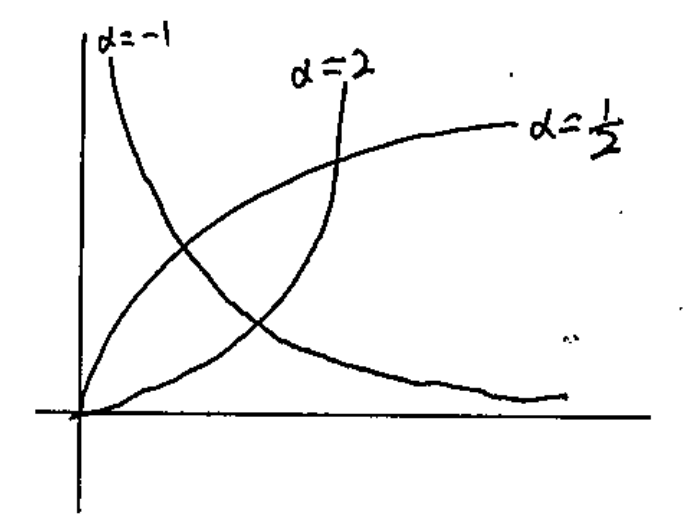
\includegraphics[width=1.8in,height=1.8in]{figures/ch08/figure1106_4.png}
	%\caption{This is an inserted JPG graphic} 
	%\label{fig:graph} 
	\end{marginfigure}
	
	\item $F(x) = \log x$, $\text{dom}\ F = \reals_{++}$, $F'(x) = \frac{1}{x}$, $F''(x) = -\frac{1}{x^2}<0$, so it is concave.
	
	\item $F(x) = x\log x$, $\text{dom}\ F = \reals_{++}$, $\frac{\alpha^2}{\alpha x^2}F(x) = \frac{\alpha}{\alpha x}[log_e(x) + \frac{x}{x}] = \frac{1}{x} > 0$, so it is convex.
	
	\item $F(x) = e^{\alpha x}$, $\text{dom}\ F = \reals$, $F''(x) = \alpha^2 e^{\alpha x}$, so it is convex for for $\alpha\neq 0$.
	
	\item $F(x) = \frac{1}{2}x^{\trans}Hx + c^{\trans}x + d$, the gradient and Hessian of $F$ are given by
	\begin{align*}
	\nabla F(x) &= \frac{1}{2}(H+H^{\trans})x + c = \tilde{H}x + c\\
	\nabla^2F(x) &= \tilde{H}
	\end{align*}
	If $\tilde{H}\geq 0$, then it is convex; If $\tilde{H}\leq 0$, then it is concave.
	
	If $\tilde{H}$ is neither PSD or negative semi-definite, then $F$ is neither convex or concave.
\end{enumerate}

\begin{example} Consider following quadratic function,
	\begin{align*}
	F(x,y) 
	&= x^2 + y^2 + 3xy \\
	&= 
	\begin{bmatrix}
	x&y
	\end{bmatrix}
	\begin{bmatrix}
	1&\frac{3}{2}\\
	\frac{3}{2} & 1
	\end{bmatrix}
	\begin{bmatrix}
	x\\
	y
	\end{bmatrix}\\
	&=\frac{1}{2}
	\begin{bmatrix}
	x&y
	\end{bmatrix}
	\begin{bmatrix}
	2&3\\
	3 & 2
	\end{bmatrix}
	\begin{bmatrix}
	x\\
	y
	\end{bmatrix}
	\end{align*}
	
	Compute the eigenvalues of the matrix, 
	\begin{align*}
	\det(
	\begin{bmatrix}
	2&3\\
	3&2
	\end{bmatrix} 
	- \lambda I) 
	&= \det
	\begin{bmatrix}
	2-\lambda & 3\\
	3 & 2-\lambda
	\end{bmatrix}\\
	&= (2-\lambda)^2 - 9\\
	&= (\lambda - 5)(\lambda + 1)
	\end{align*}
	
	The matrix has one negative eigenvalue and one positive eigenvalue, so it is neither PSD or negative PSD.
	
	Also, if we try $-45^{\circ}$ line, we will see slice is not convex,
	$$F(x,-x) = x^2 + (-x)^2 + 3x(-x) = 2x^2 - 3x^2 = -x^2.$$
	
\end{example}

\begin{example}
	Geometric mean $\sqrt{x_1x_2} = F(x_1,x_2)$, $\text{dom}\ F = \reals_+ \times \reals_+$, is concave. 
	
	The Hessian of $F$ is given by
	\begin{equation*}
	\nabla^2F(x) = -\frac{\sqrt{x_1x_2}}{y}\begin{bmatrix}
	\frac{1}{x^2_1} & -\frac{1}{x_1x_2}\\
	-\frac{1}{x_1x_2} & \frac{1}{x^2_2}
	\end{bmatrix}
	\end{equation*}
	
	There are two ways to determine the type of the Hessian(e.g., whether it is PSD)
	
	1) Calculate eigenvalues as we did in previous example.
	
	2) Use definition of negative PSD (or PSD):
	\begin{align*}
	v^{\trans}\nabla^2F(x)v &= -\frac{\sqrt{x_1x_2}}{2}[\frac{v_1^2}{x_1^2} - \frac{2v_1v_2}{x_1x_2} + \frac{v_2^2}{x^2_2}]\\
	&= -\frac{\sqrt{x_1x_2}}{2}(\frac{v_1}{x_1} -\frac{v_2}{x_2}) \leq 0
	\end{align*}
	
	So it is concave in $(x_1, x_2)$. More generally, the function $F(x) = (\prod^n_{i=1}x_i)^{\frac{1}{n}}$ is concave in $x\in \reals^n$.
\end{example}

\subsection{Consequence of convexity conditions for differentiable $F$}

\quad By first order condition, if $F$ is convex, then we have
$$F(y)\geq F(x) + \nabla F(x)^{\trans}(y-x), \forall x,y\in \text{dom}\ F$$

What if $\nabla F(x^*) = 0 \in \reals^n$ for some $x^*\in \text{dom}\ F$? In this case we may have
$$F(y)\geq F(x^*) + \nabla F(x^*)^{\trans}(y-x^*)=F(x^*),\ \forall y\in \text{dom}\ F$$

Therefore, if we can find an $x^*\in \text{dom}\ F$ such that $\nabla F(x^*) = 0$, then it is also a global minimum.

%Above are notes for Nov 6



%Below are notes for Nov 11

\subsection{Local minima vs Global minima}

\begin{marginfigure}
	\centering
	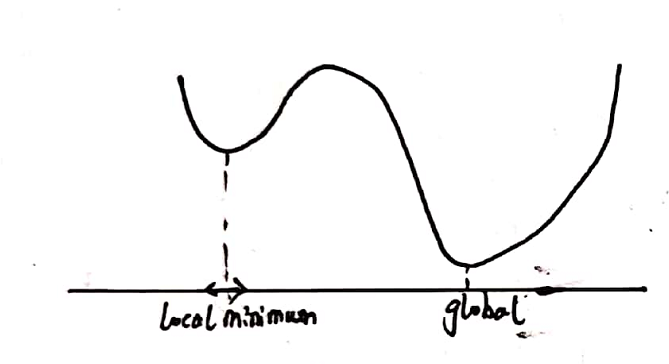
\includegraphics[width=1.8in,height=1.8in]{figures/ch08/figure1111_1.png}
	%\caption{This is an inserted JPG graphic} 
	%\label{fig:graph} 
\end{marginfigure}

\begin{definition}
	$x^*$ is a local minimum of $F$ if $\exists \epsilon >0$ such that for all $x$ satisfying $\Vert x - x^*\Vert < \epsilon$ we will have $F(x) \geq F(x^*)$.
\end{definition}

\begin{theorem}
	Suppose $F$ is twice differentiable (not necessarily to be convex), then we have
	
	(1) If $x^*$ is a local optimum, then $\nabla F(x^*) = 0$ and $\nabla^2F(x^*)\geq 0$.
	
	(2) If $\nabla F(x^*) = 0$ and $\nabla^2F(x^*)> 0$, then $x^*$ is a local minimum. 
\end{theorem}

%Consider:
%
%\begin{align*}
%&F(x) = x^3 \quad \text{at} \quad x = 0\\
%&F'(x) = 3x^2 \quad \text{at} \quad F'(0) = 0\\
%&F''(x) = 6x \quad \text{at} \quad F''(0) = 0
%\end{align*}

\begin{proof}[Proof of (1)]
	Let $x^*$ be a local optimum, consider any $v$:
	\begin{equation*}
	lim_{t\rightarrow 0^+}\frac{F(x^* + tv) - F(x^*)}{t} = \nabla F(x^*)^{\trans}v\geq 0
	\end{equation*}
	It's non-negative since $x^*$ is local minimum.
	
	This implies that $\nabla F(x^*) = 0$ because $v$ is arbitrary. 
	
	E.g. If $\nabla F(x^*) \neq 0$, then take $v = -\nabla F(x^*)$ and we would get a negative one unless $\nabla F(x^*) = 0.$
	
Consider the second derivative,
\begin{align*}
lim_{t\rightarrow 0^+}\frac{F(x^* + tv) - F(x^*)}{t^2} &= lim_{t\rightarrow 0^+} \frac{F(x^*) + \nabla F(x^*)^{\trans}(tv) + \frac{1}{2}(tv)^{\trans}\nabla F(x^*)(tv) + o(t^2) - F(x^*)}{t^2}\\
&= lim_{t\rightarrow 0^+} \frac{1}{2}v^{\trans}\nabla^2F(x^*)v+\frac{\sigma(t^2)}{t^2}\\
&= \frac{1}{2}v^{\trans}\nabla^2F(x^*)v \\
&\geq 0
\end{align*}

Since $v$ is arbitrary and by definition of PSD, the Hessian $\nabla^2 F(x^*) \geq 0$

\end{proof}

For twice differentiable functions, what we are told here is: 

$x^*$ is a local optimum $\Rightarrow$ $\nabla F(x^*) = 0$ and $\nabla^2F(x^*)\geq 0$.

Furthermore, if the function $F$ is convex, we may have

$\Rightarrow$ $\nabla^2F(x)\geq0, \forall x\in \text{dom}F$

$\Rightarrow$ $\nabla F(x^*) = 0$ $\Rightarrow$ $x^*$ is global optimum.

Put together to say: If $F$ is convex, then the local optimum is also the global optimum.\\

\vspace{0.3cm}

\begin{proof}[Proof of (2)]
	If $\nabla F(x^*) = 0$ and $\nabla^2 F(x^*) > 0$, then $x^*$ is a local optimum.
	
	Again, use Taylor expansion: 
	\begin{align*}
	F(x) &= F(x^* + tv) \\
	&= F(x^*) + \nabla F(x^*)^{\trans}(tv) + \frac{1}{2}(tv)^{\trans}\nabla^2F(x^*)(tv) + o(\Vert v \Vert^2)\\
	&= F(x^*) + \frac{1}{2}t^2v^{\trans}\nabla^2F(x^*)v + o(\Vert v \Vert^2)
	\end{align*}
	
	$\Rightarrow$ If $t$ is sufficiently small, the quadratic term dominates the $o(\Vert v \Vert^2)$ term.
	
	$\Rightarrow$ Any point in neighborhood sufficiently small (meaning $t$ sufficiently small) has evaluation larger than $F(x^*)$.
	
	$\Rightarrow$ $x^*$ is local optimum. 
\end{proof}

\textbf{Remarks: }
\begin{enumerate}
	\item It is possible that there is no local or global optimum.
	
	\begin{marginfigure}
	\centering
	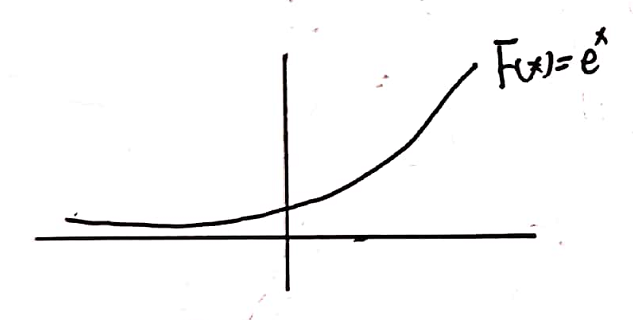
\includegraphics[width=1.8in,height=1.8in]{figures/ch08/figure1111_2.png}
	%\caption{This is an inserted JPG graphic} 
	%\label{fig:graph} 
	\end{marginfigure}
	
	This graph is on $\inf\, F(x) = 0$ but there is no $x\in \text{dom}F = \reals$ achieves $F(x) = 0$.
	
	\item The above story is for unconstrained optimization problem, since we consider the entire domain above.
	
	\begin{marginfigure}
	\centering
	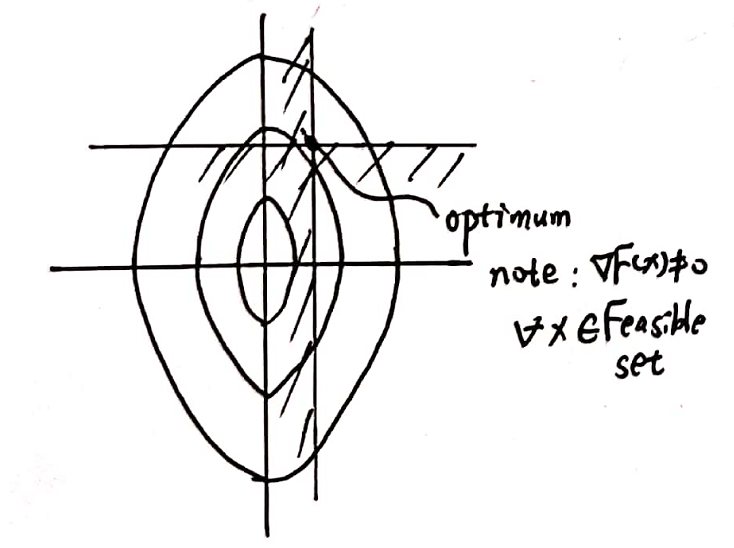
\includegraphics[width=1.8in,height=1.8in]{figures/ch08/figure1111_3.png}
	%\caption{This is an inserted JPG graphic} 
	%\label{fig:graph} 
	\end{marginfigure}
	
\end{enumerate}






\vspace{0.5cm}
\subsection{Composition of Functions}

Let $F(x) = h(g(x))$ where $g: \reals^n \rightarrow \reals$ and $h: \reals\rightarrow \reals$. Then $F: \reals^n\rightarrow \reals$ is convex if:



\begin{enumerate}
	\item $g$ is convex, $h$ is convex and non-decreasing. Or,
	
	\item $g$ is concave, $h$ is convex and non-increasing.
\end{enumerate}

\begin{marginfigure}
	\centering
	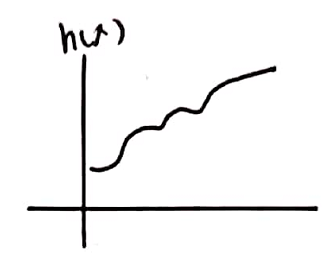
\includegraphics[width=1.8in,height=1.8in]{figures/ch08/figure1111_4.png}
	%\caption{This is an inserted JPG graphic} 
	%\label{fig:graph} 
\end{marginfigure}

\begin{marginfigure}
	\centering
	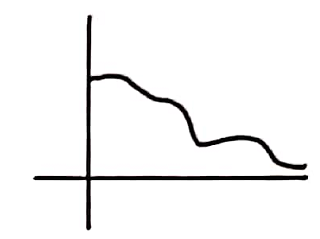
\includegraphics[width=1.8in,height=1.8in]{figures/ch08/figure1111_5.png}
	%\caption{This is an inserted JPG graphic} 
	%\label{fig:graph} 
\end{marginfigure}

Prove: For differentiable functions, can also prove for non-differentiable. 

(i)

\begin{itemize}
	\item $F'(x) = h'(g(x))g'(x)$.
	
	\item $F''(x) = h''(g(x))g'(x)g'(x) + h'(g(x))g''(x) \geq 0$ 
\end{itemize}



Note: Doing derivative for $n=1$ without loss of generality because we showed a convex function must be convex along all lines. 



(ii) 
\begin{equation*}
F''(x) = h''(g(x))(g'(x))^2 + h'(g(x))g''(x) \geq 0
\end{equation*}

Can extend to multiple dimensions.
\begin{align*}
&g_i:\reals^n\rightarrow \reals, h:\reals^k\rightarrow \reals\\
F(x) &= h(g(x))\\
&= h(g_1(x) g_2(x)...g_k(x)) \text{is convex}
\end{align*}

$\cdot$ $g$ is convex and $h$ is convex and non-decreasing in each of its arguments. 



\begin{example}
	
	The function $F(x) = \exp(g(x))$ is convex, where $g(x)$ is convex. 
	
	Apparently we could let $h(\cdot) = \exp(\cdot)$, and since it is convex and non-decreasing, $F(x)$ is convex. 
\end{example}


\begin{example}
	
	The function $F(x) = \frac{1}{g(x)}$ is convex if $g(x)$ is concave and positive, $\forall x$. 
	
	We let $F(x) = h(g(x))$, where $h(x) = \frac{1}{x}$. Since $\text{dom}\ h = \reals_{++}$, $h$ is convex.
	
	Note that $h$ is convex and $h(x) = \frac{1}{x}$ is non-increasing on $\reals_{++}$, so if $g(\cdot)$ is concave, then $F$ is a convex function.
\end{example}


\begin{example}
	The function $F(x) = -\sum^k_{i=1}log(-F_i(x))$ is convex on $\{x\vert F_i(x)<0\ \forall i\in \{1,\cdots,k \}  \}$ if all $F_i$ are convex.
	
	Consider the domain of this $F$, note that for each $F_i(x)<0\Leftrightarrow -F_i(x) >0$, so $\text{dom}\ F = \cap^k_{i=1}\{x\vert F_i(x) <0 \}$. It is the intersection of sublevel sets of convex functions, and therefore it is a convex set.
		
	Since $F(x) = \sum^k_{i=1} -log(-F_i(x))$ is the positive sum of convex functions, it is convex eventually.
\end{example}
